% Options for packages loaded elsewhere
\PassOptionsToPackage{unicode}{hyperref}
\PassOptionsToPackage{hyphens}{url}
%
\documentclass[
]{book}
\usepackage{amsmath,amssymb}
\usepackage{iftex}
\ifPDFTeX
  \usepackage[T1]{fontenc}
  \usepackage[utf8]{inputenc}
  \usepackage{textcomp} % provide euro and other symbols
\else % if luatex or xetex
  \usepackage{unicode-math} % this also loads fontspec
  \defaultfontfeatures{Scale=MatchLowercase}
  \defaultfontfeatures[\rmfamily]{Ligatures=TeX,Scale=1}
\fi
\usepackage{lmodern}
\ifPDFTeX\else
  % xetex/luatex font selection
\fi
% Use upquote if available, for straight quotes in verbatim environments
\IfFileExists{upquote.sty}{\usepackage{upquote}}{}
\IfFileExists{microtype.sty}{% use microtype if available
  \usepackage[]{microtype}
  \UseMicrotypeSet[protrusion]{basicmath} % disable protrusion for tt fonts
}{}
\makeatletter
\@ifundefined{KOMAClassName}{% if non-KOMA class
  \IfFileExists{parskip.sty}{%
    \usepackage{parskip}
  }{% else
    \setlength{\parindent}{0pt}
    \setlength{\parskip}{6pt plus 2pt minus 1pt}}
}{% if KOMA class
  \KOMAoptions{parskip=half}}
\makeatother
\usepackage{xcolor}
\usepackage{longtable,booktabs,array}
\usepackage{calc} % for calculating minipage widths
% Correct order of tables after \paragraph or \subparagraph
\usepackage{etoolbox}
\makeatletter
\patchcmd\longtable{\par}{\if@noskipsec\mbox{}\fi\par}{}{}
\makeatother
% Allow footnotes in longtable head/foot
\IfFileExists{footnotehyper.sty}{\usepackage{footnotehyper}}{\usepackage{footnote}}
\makesavenoteenv{longtable}
\usepackage{graphicx}
\makeatletter
\def\maxwidth{\ifdim\Gin@nat@width>\linewidth\linewidth\else\Gin@nat@width\fi}
\def\maxheight{\ifdim\Gin@nat@height>\textheight\textheight\else\Gin@nat@height\fi}
\makeatother
% Scale images if necessary, so that they will not overflow the page
% margins by default, and it is still possible to overwrite the defaults
% using explicit options in \includegraphics[width, height, ...]{}
\setkeys{Gin}{width=\maxwidth,height=\maxheight,keepaspectratio}
% Set default figure placement to htbp
\makeatletter
\def\fps@figure{htbp}
\makeatother
\setlength{\emergencystretch}{3em} % prevent overfull lines
\providecommand{\tightlist}{%
  \setlength{\itemsep}{0pt}\setlength{\parskip}{0pt}}
\setcounter{secnumdepth}{5}
% definitions for citeproc citations
\NewDocumentCommand\citeproctext{}{}
\NewDocumentCommand\citeproc{mm}{%
  \begingroup\def\citeproctext{#2}\cite{#1}\endgroup}
\makeatletter
 % allow citations to break across lines
 \let\@cite@ofmt\@firstofone
 % avoid brackets around text for \cite:
 \def\@biblabel#1{}
 \def\@cite#1#2{{#1\if@tempswa , #2\fi}}
\makeatother
\newlength{\cslhangindent}
\setlength{\cslhangindent}{1.5em}
\newlength{\csllabelwidth}
\setlength{\csllabelwidth}{3em}
\newenvironment{CSLReferences}[2] % #1 hanging-indent, #2 entry-spacing
 {\begin{list}{}{%
  \setlength{\itemindent}{0pt}
  \setlength{\leftmargin}{0pt}
  \setlength{\parsep}{0pt}
  % turn on hanging indent if param 1 is 1
  \ifodd #1
   \setlength{\leftmargin}{\cslhangindent}
   \setlength{\itemindent}{-1\cslhangindent}
  \fi
  % set entry spacing
  \setlength{\itemsep}{#2\baselineskip}}}
 {\end{list}}
\usepackage{calc}
\newcommand{\CSLBlock}[1]{\hfill\break\parbox[t]{\linewidth}{\strut\ignorespaces#1\strut}}
\newcommand{\CSLLeftMargin}[1]{\parbox[t]{\csllabelwidth}{\strut#1\strut}}
\newcommand{\CSLRightInline}[1]{\parbox[t]{\linewidth - \csllabelwidth}{\strut#1\strut}}
\newcommand{\CSLIndent}[1]{\hspace{\cslhangindent}#1}
\ifLuaTeX
  \usepackage{selnolig}  % disable illegal ligatures
\fi
\usepackage{bookmark}
\IfFileExists{xurl.sty}{\usepackage{xurl}}{} % add URL line breaks if available
\urlstyle{same}
\hypersetup{
  pdftitle={Metodologia científica e Bioestatística},
  pdfauthor={Editor: Dr.~Hércules Rezende Freitas},
  hidelinks,
  pdfcreator={LaTeX via pandoc}}

\title{Metodologia científica e Bioestatística}
\author{Editor: Dr.~Hércules Rezende Freitas}
\date{2024-11-29}

\begin{document}
\maketitle

{
\setcounter{tocdepth}{1}
\tableofcontents
}
\chapter{Sobre o projeto}\label{sobre-o-projeto}

O projeto ``Metodologia científica e Bioestatística'' é colaborativo e de acesso aberto. O objetivo é que o documento seja sempre atualizado e que seus autores sejam reconhecidos por suas contribuições.

\chapter{Introdução à metodologia científica}\label{introduuxe7uxe3o-uxe0-metodologia-cientuxedfica}

\section{Conceitos básicos de ciência}\label{conceitos-buxe1sicos-de-ciuxeancia}

\section{O método científico}\label{o-muxe9todo-cientuxedfico}

\section{Paradigmas científicos}\label{paradigmas-cientuxedficos}

\section{Ética na pesquisa científica}\label{uxe9tica-na-pesquisa-cientuxedfica}

\chapter{Formulação de problemas e hipóteses}\label{formulauxe7uxe3o-de-problemas-e-hipuxf3teses}

\section{Identificação de problemas de pesquisa}\label{identificauxe7uxe3o-de-problemas-de-pesquisa}

\section{Revisão da literatura}\label{revisuxe3o-da-literatura}

\section{Definição de objetivos}\label{definiuxe7uxe3o-de-objetivos}

\section{Formulação de hipóteses}\label{formulauxe7uxe3o-de-hipuxf3teses}

\chapter{Desenhos de pesquisa}\label{desenhos-de-pesquisa}

\section{Estudos observacionais}\label{estudos-observacionais}

\subsection{Estudos transversais}\label{estudos-transversais}

\subsection{Estudos de coorte}\label{estudos-de-coorte}

\subsection{Estudos de caso-controle}\label{estudos-de-caso-controle}

\section{Ensaios clínicos}\label{ensaios-cluxednicos}

\subsection{Ensaios randomizados controlados}\label{ensaios-randomizados-controlados}

\subsection{Estudos duplo-cegos}\label{estudos-duplo-cegos}

\section{Estudos experimentais}\label{estudos-experimentais}

\subsection{Desenho experimental}\label{desenho-experimental}

\subsection{Controle e aleatorização}\label{controle-e-aleatorizauxe7uxe3o}

\chapter{Bioestatística descritiva}\label{bioestatuxedstica-descritiva}

\section{Medidas de tendência central}\label{medidas-de-tenduxeancia-central}

\subsection{Média}\label{muxe9dia}

\subsection{Mediana}\label{mediana}

\subsection{Moda}\label{moda}

\section{Medidas de dispersão}\label{medidas-de-dispersuxe3o}

\subsection{Variância}\label{variuxe2ncia}

\subsection{Desvio padrão}\label{desvio-padruxe3o}

\subsection{Amplitude}\label{amplitude}

\section{Distribuições de frequência}\label{distribuiuxe7uxf5es-de-frequuxeancia}

\section{Representações gráficas}\label{representauxe7uxf5es-gruxe1ficas}

\subsection{Histogramas}\label{histogramas}

\subsection{Boxplots}\label{boxplots}

\subsection{Gráficos de dispersão}\label{gruxe1ficos-de-dispersuxe3o}

\chapter{Bioestatística inferencial}\label{bioestatuxedstica-inferencial}

\section{Conceitos de probabilidade}\label{conceitos-de-probabilidade}

\section{Distribuições de probabilidade}\label{distribuiuxe7uxf5es-de-probabilidade}

\subsection{Distribuição normal}\label{distribuiuxe7uxe3o-normal}

\subsection{Distribuição t de student}\label{distribuiuxe7uxe3o-t-de-student}

\subsection{Distribuição qui-quadrado}\label{distribuiuxe7uxe3o-qui-quadrado}

\section{Estimação e intervalos de confiança}\label{estimauxe7uxe3o-e-intervalos-de-confianuxe7a}

\section{Testes de hipóteses}\label{testes-de-hipuxf3teses}

\subsection{Testes paramétricos}\label{testes-paramuxe9tricos}

\subsection{Testes não-paramétricos}\label{testes-nuxe3o-paramuxe9tricos}

\chapter{Análise de dados}\label{anuxe1lise-de-dados}

\section{Correlação e regressão}\label{correlauxe7uxe3o-e-regressuxe3o}

\subsection{Correlação de Pearson e Spearman}\label{correlauxe7uxe3o-de-pearson-e-spearman}

\subsection{Regressão linear simples e múltipla}\label{regressuxe3o-linear-simples-e-muxfaltipla}

\section{Análise de variância (ANOVA)}\label{anuxe1lise-de-variuxe2ncia-anova}

\subsection{ANOVA de uma via}\label{anova-de-uma-via}

\subsection{ANOVA fatorial}\label{anova-fatorial}

\section{Análise multivariada}\label{anuxe1lise-multivariada}

\subsection{Componentes principais}\label{componentes-principais}

\subsection{Clusterização}\label{clusterizauxe7uxe3o}

\chapter{\texorpdfstring{Uso de \emph{softwares} estatísticos}{Uso de softwares estatísticos}}\label{uso-de-softwares-estatuxedsticos}

\section{\texorpdfstring{\emph{Softwares} ``no-code'' e ``low-code''}{Softwares ``no-code'' e ``low-code''}}\label{softwares-no-code-e-low-code}

\section{R para análise estatística}\label{r-para-anuxe1lise-estatuxedstica}

Dr.~Hércules Freitas\(^1\)

\(^1\)Universidade Federal do Rio de Janeiro (UFRJ), Centro de Ciências da Saúde, Instituto de Bioquímica Leopoldo de Meis, Laboratório de Erros Inatos do Metabolismo, Rio de Janeiro/RJ, Brasil.

\subsection{Aprendendo a programar}\label{aprendendo-a-programar}

Aprender a programar, especialmente em uma linguagem como R, destinada à ciência de dados, é uma jornada empolgante, mas também repleta de desafios. Um dos maiores obstáculos que os iniciantes enfrentam não é a complexidade dos conceitos ou a sintaxe da linguagem, mas a frustração que surge ao encontrar erros e \emph{bugs}. Este sentimento, embora desagradável, é uma parte integral do processo de aprendizado. A chave para superar essa frustração não está em evitá-la, mas em aprender a lidar com ela de maneira produtiva.

\subsubsection{A importância de lidar com a frustração}\label{a-importuxe2ncia-de-lidar-com-a-frustrauxe7uxe3o}

A frustração, embora desconfortável, é um sinal de que você está se desafiando e saindo da sua zona de conforto. É um indicativo de crescimento e aprendizado. Quando você se depara com um erro em seu código R, é fácil sentir-se desanimado ou questionar suas habilidades. No entanto, é crucial reconhecer que até os programadores mais experientes enfrentam erros e \emph{bugs} regularmente. A diferença está em como eles reagem a esses contratempos.

Uma habilidade subestimada na programação é a capacidade de ler e interpretar mensagens de erro. Em R, como em muitas outras linguagens de programação, as mensagens de erro são projetadas para guiar o programador na identificação e correção de problemas. Embora possam parecer crípticas no início, com a prática, você começará a reconhecer padrões comuns e entender melhor o que essas mensagens estão tentando comunicar. Abaixo, seguem algumas dicas para lidar com as dificuldades no aprendizado inicial:

\begin{enumerate}
\def\labelenumi{\arabic{enumi}.}
\item
  \textbf{Aceitação}: aceite que a frustração é uma parte normal do processo de aprendizado. Reconheça seus sentimentos, mas não permita que eles dominem sua motivação para aprender;
\item
  \textbf{Pausas estratégicas}: quando se sentir sobrecarregado, faça uma pausa. Distanciar-se temporariamente do problema pode ajudar a clarear sua mente e trazer novas perspectivas;
\item
  \textbf{Comunidade e suporte}: não hesite em buscar ajuda. A comunidade R é vasta e acolhedora, com fóruns e grupos dedicados a ajudar programadores de todos os níveis. Compartilhar suas dificuldades e buscar conselhos pode ser incrivelmente útil;
\item
  \textbf{Prática e persistência}: a prática contínua é fundamental. Quanto mais você se expõe a diferentes problemas e erros, mais equipado estará para lidar com eles no futuro;
\item
  \textbf{Celebre pequenas vitórias}: cada erro corrigido é um passo à frente em sua jornada de aprendizado. Celebre essas conquistas e reconheça seu progresso.
\end{enumerate}

Aprender a programar em R é uma jornada valiosa que abre portas para o mundo da análise de dados. Embora a frustração seja uma parte inevitável desse processo, adotar uma abordagem positiva e resiliente pode transformar esses desafios em oportunidades de aprendizado. Lembre-se, cada erro é uma chance de crescer, e cada problema resolvido é um passo em direção à maestria na programação. Mantenha-se motivado, pratique regularmente e, mais importante, seja paciente consigo mesmo. O caminho para se tornar proficiente em R pode ser longo, mas é, sem dúvida, recompensador.

\subsection{Visão geral do R e suas aplicações}\label{visuxe3o-geral-do-r-e-suas-aplicauxe7uxf5es}

R é uma linguagem de programação e um ambiente de software para análise estatística e gráfica. A história do R remonta à década de 1970 com o desenvolvimento da linguagem S no Bell Labs por John Chambers e outros (\citeproc{ref-chambers1980}{Chambers 1980}). A linguagem S foi projetada para ser uma linguagem de programação que fosse tanto eficiente quanto fácil de usar, com foco em análise de dados e gráficos estatísticos.

Na década de 1990, Ross Ihaka e Robert Gentleman, da Universidade de Auckland, na Nova Zelândia, iniciaram o desenvolvimento do R como um projeto de pesquisa. Eles foram influenciados pela linguagem S e pelo Scheme, uma linguagem de programação com semântica de escopo léxico. O R foi concebido como um dialeto da linguagem S, com a intenção de melhorar e ampliar a análise estatística e as capacidades gráficas (\citeproc{ref-ihaka1996}{Ihaka and Gentleman 1996}).

R é uma linguagem de programação interpretada, o que significa que o código é executado diretamente, sem a necessidade de compilação prévia. Isso facilita a depuração e o desenvolvimento iterativo. Além disso, R é uma linguagem dinamicamente tipada, permitindo que os tipos de dados sejam alterados em tempo de execução.

Uma das principais características do R é a sua extensibilidade. A comunidade de usuários e desenvolvedores contribuiu com uma vasta coleção de pacotes que estendem a funcionalidade básica do R, disponíveis através do \emph{Comprehensive R Archive Network (CRAN)} (\citeproc{ref-hornik2012}{Hornik 2012}). Esses pacotes cobrem uma ampla gama de técnicas estatísticas, modelos gráficos, métodos de \emph{machine learning}, e muito mais.

R também é conhecido por sua capacidade de produzir gráficos de alta qualidade, que são essenciais para a análise exploratória de dados e a apresentação de resultados estatísticos. A linguagem oferece diversas funções e pacotes para a criação de gráficos, incluindo o popular \emph{ggplot2}, que permite a construção de gráficos complexos de maneira intuitiva (\citeproc{ref-wickham2011}{Wickham 2011}).

Outra característica importante do R é a sua comunidade ativa e colaborativa. Os usuários de R frequentemente compartilham seu código e experiências, ajudando uns aos outros a resolver problemas e a melhorar suas habilidades de programação. Isso é facilitado por fóruns de discussão, listas de e-mail e conferências.

As principais aplicações da linguagem R no mundo do trabalho abrangem uma vasta gama de setores, especialmente aqueles que dependem intensamente da análise de dados, estatística e modelagem preditiva. Profissões como cientistas de dados, analistas de mercado, pesquisadores em saúde e biologia, e especialistas em \emph{machine learning} são apenas alguns exemplos de carreiras que se beneficiam diretamente do uso de R. Esta linguagem é particularmente valorizada por sua capacidade de manipular grandes conjuntos de dados, realizar análises estatísticas complexas, criar visualizações de dados avançadas e desenvolver modelos de \emph{machine learning}.

No futuro, espera-se que a demanda por profissionais com habilidades em R continue a crescer, à medida que mais setores reconhecem a importância da tomada de decisões baseada em dados. Profissões emergentes, como especialistas em big data, analistas de cibersegurança que utilizam técnicas de aprendizado de máquina para identificar ameaças, e profissionais envolvidos na criação e gestão de ambientes virtuais no metaverso, também poderão se beneficiar do uso de R.

Além disso, à medida que a inteligência artificial (IA) e a análise de dados se tornam cada vez mais integradas em diferentes aspectos do mundo do trabalho, a capacidade de utilizar R para desenvolver e implementar soluções baseadas em dados será uma habilidade altamente valorizada.

A linguagem R, com sua comunidade ativa e vasta coleção de pacotes, oferece uma plataforma robusta para inovação e desenvolvimento em diversas áreas. Profissionais do futuro poderão utilizar R para explorar novos territórios em ciência de dados, otimização de processos, desenvolvimento de produtos baseados em IA, análises ambientais e muito mais. A flexibilidade e a capacidade de adaptação de R a diferentes contextos e desafios tornam-na uma ferramenta valiosa para profissionais que buscam estar na vanguarda da inovação e da análise de dados.

\subsection{\texorpdfstring{\textbf{Instalando o R e o RStudio}~}{Instalando o R e o RStudio~}}\label{instalando-o-r-e-o-rstudio}

Para instalar o R e o RStudio em computadores com sistemas operacionais Windows ou Mac, siga os passos abaixo:~~

\subsubsection{Instalação do R no Windows:~}\label{instalauxe7uxe3o-do-r-no-windows}

\begin{enumerate}
\def\labelenumi{\arabic{enumi}.}
\item
  Acesse o site do CRAN (\href{https://cran.r-project.org}{Comprehensive R Archive Network}), que é uma rede de servidores que armazena versões atualizadas do R;~
\item
  Em ``\emph{Download and Install R}'', clique em ``\emph{Download R for Windows}'';~
\item
  Clique em ``\emph{\ldots install R for the first time}'';
\item
  Clique em ``\emph{Download R x.x.x for Windows}'', onde ``x.x.x'' é o número da versão mais recente;

  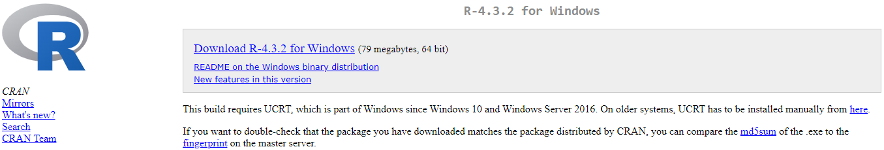
\includegraphics{images/clipboard-1429771558.png}
\item
  Após o \emph{download}, execute o arquivo baixado e siga as instruções do instalador. Durante a instalação, você pode aceitar as configurações padrão, que são adequadas para a maioria dos usuários.
\end{enumerate}

\subsubsection{Instalação do RStudio no Windows}\label{instalauxe7uxe3o-do-rstudio-no-windows}

\begin{enumerate}
\def\labelenumi{\arabic{enumi}.}
\item
  Após instalar o R, acesse o site do \href{https://posit.co/download/rstudio-desktop/}{RStudio (Posit)};
\item
  Desça a página e clique em ``\emph{Download RStudio Desktop for Windows}'';

  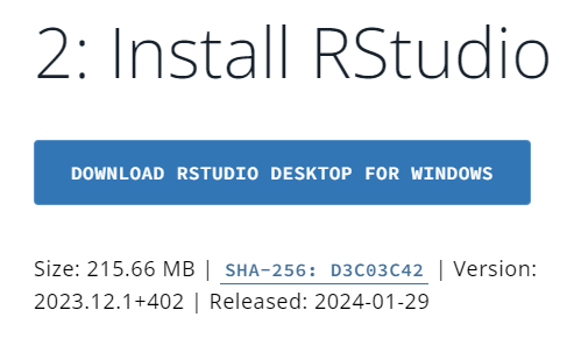
\includegraphics[width=3.47917in,height=\textheight]{images/clipboard-3306259698.png}
\item
  Execute o arquivo baixado e siga as instruções para concluir a instalação.
\end{enumerate}

\subsubsection{Instalação do R no Mac}\label{instalauxe7uxe3o-do-r-no-mac}

\begin{enumerate}
\def\labelenumi{\arabic{enumi}.}
\item
  Acesse o site do \href{https://cran.r-project.org}{CRAN};
\item
  Clique em ``\emph{Download R for macOS}'';

  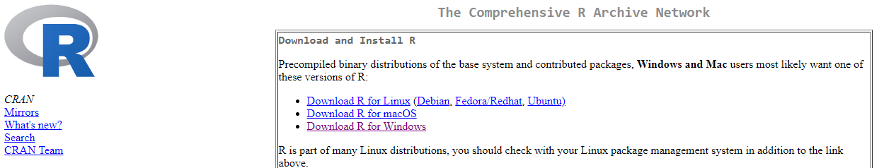
\includegraphics{images/clipboard-2368293499.png}
\item
  Escolha a versão do R que deseja instalar (\emph{Macbooks Intell, mais antigos, ou Macbooks M1/M2});

  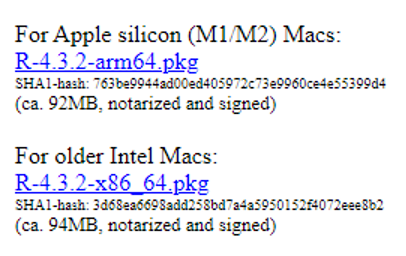
\includegraphics[width=2.69792in,height=\textheight]{images/clipboard-3553229090.png}
\item
  Após o \emph{download}, abra o arquivo ``.pkg'' baixado e siga as instruções para instalar o R.
\end{enumerate}

\subsubsection{Instalação do RStudio no Mac}\label{instalauxe7uxe3o-do-rstudio-no-mac}

\begin{enumerate}
\def\labelenumi{\arabic{enumi}.}
\item
  Visite o site do \href{https://posit.co/download/rstudio-desktop/}{RStudio (Posit)} após instalar o R;
\item
  Clique em ``\emph{Download RStudio}'';
\item
  Na seção \emph{RStudio Desktop}, clique em ``\emph{Download RStudio Desktop for Mac}'';
\item
  Escolha a versão apropriada para Mac, seja para processadores Intel ou M1, e inicie o \emph{download};
\item
  Abra o arquivo baixado e siga as instruções para instalar o RStudio.
\end{enumerate}

Após a instalação, você estará pronto(a) para utilizar todas as funcionalidades do R no RStudio.

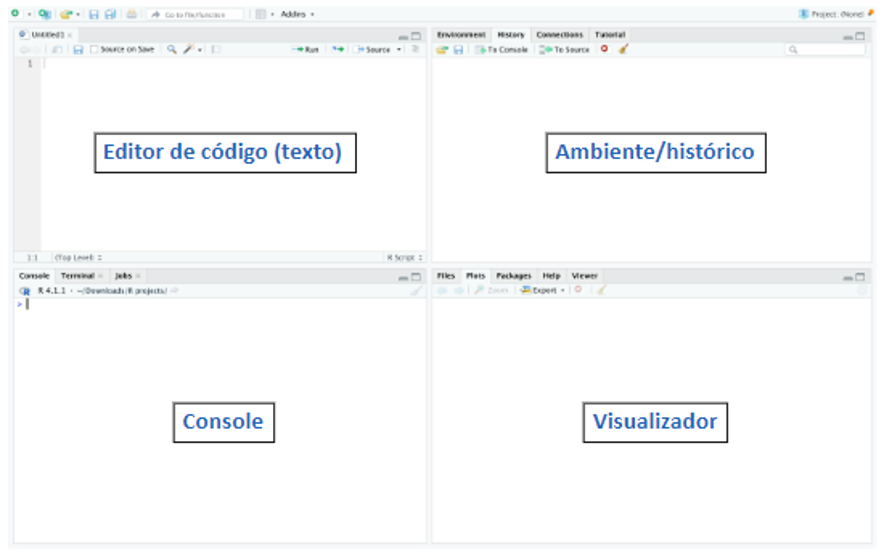
\includegraphics[width=5.25in,height=\textheight]{images/clipboard-4172689374.png}

\subsection{Sintaxe básica e operações no R}\label{sintaxe-buxe1sica-e-operauxe7uxf5es-no-r}

\subsubsection{Sintaxe básica}\label{sintaxe-buxe1sica}

A sintaxe do R é bastante simples e direta. A linguagem faz distinção entre maiúsculas e minúsculas, portanto, ``A'' e ``a'' são considerados símbolos diferentes e podem se referir a variáveis diferentes. Os comandos no R são expressões ou atribuições. Se um comando é uma expressão, seu valor é calculado e visualizado, mas é perdido em seguida. Uma atribuição, por outro lado, calcula a expressão e atribui o resultado a uma variável, que é salva no ambiente de trabalho do R. Aqui está um exemplo de atribuição a variável no R (``x \textless- 1'' ou ``x é igul a 1''):

\textbf{Passo 1}: digite o código desejado no editor

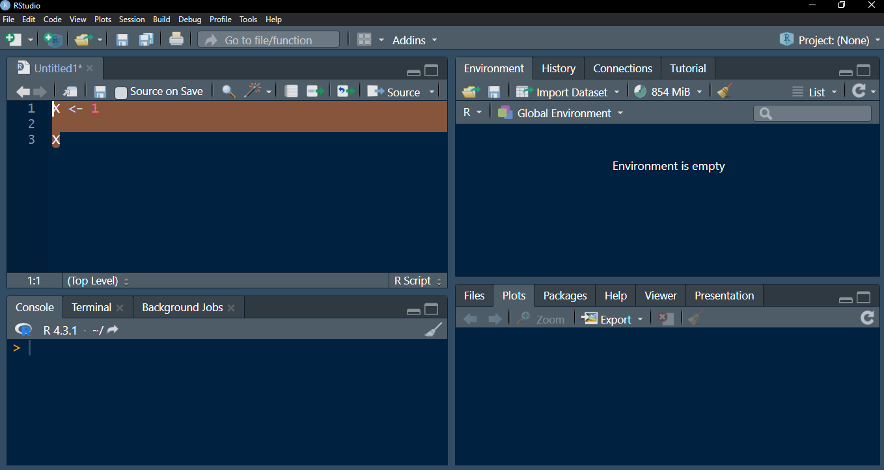
\includegraphics{images/clipboard-474586210.png}

* O código acima indica, na primeira linha, ``X contém o valor 1''. A segunda linha ``pede'' ao programa que indique o valor de ``X''.

\textbf{Passo 2}: selecione o código a ser executado e aperte ``Ctrl + Enter''

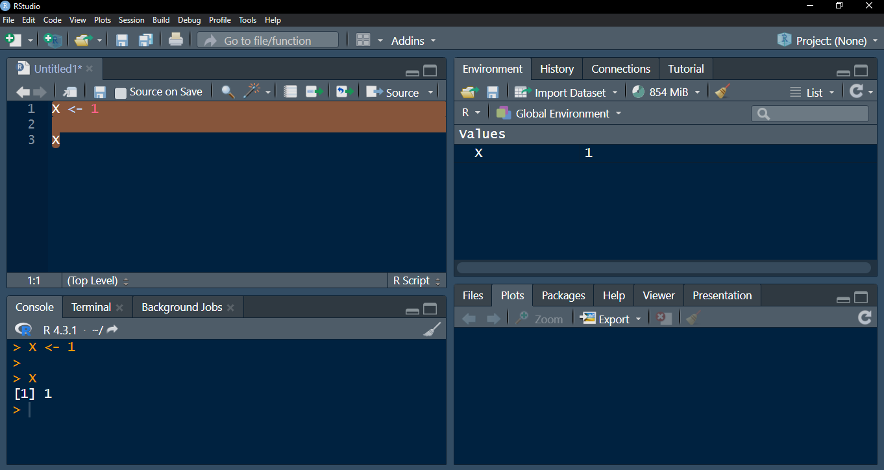
\includegraphics{images/clipboard-2485386777.png}

*O resultado é apresentado no Console (i.e., ``{[}1{]} 1'' ou ``X contém um valor, e esse valor é 1'').

\textbf{Passo 3}: use o objeto X gerado em outros códigos

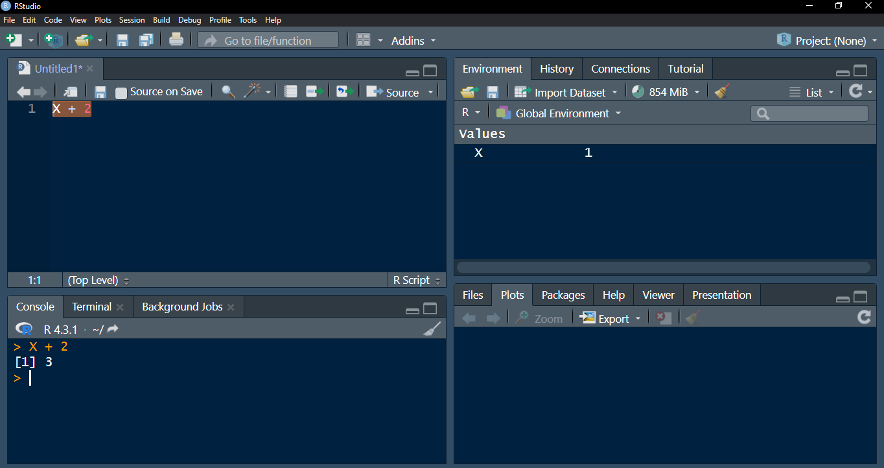
\includegraphics{images/clipboard-3669577123.png}

*''X'' é um objeto de valor 1. Se somado a 2, retorna o valor 3.

Agora, tente interagir com os exemplos abaixo:

\begin{enumerate}
\def\labelenumi{\arabic{enumi}.}
\item
  \textbf{Criação de vetores}: v \textless- c(1, 2, 3, 4, 5)
\item
  \textbf{Criação de matrizes}: m \textless- matrix(1:9, nrow = 3, ncol = 3)
\item
  \textbf{Criação de listas}: l \textless- list(nome = ``João'', idade = 30, altura = 1.75)
\item
  \textbf{Criação de data frames}: df \textless- data.frame(nome = c(``João'', ``Maria''), idade = c(30, 25))
\end{enumerate}

\textbf{Exemplo}: produzindo um \emph{data frame} (quadro de dados)

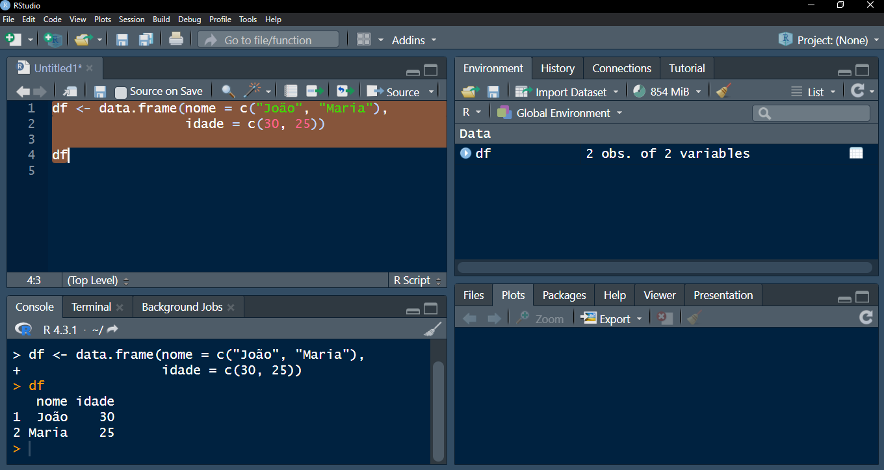
\includegraphics{images/clipboard-3472985925.png}

\subsubsection{Operações básicas}\label{operauxe7uxf5es-buxe1sicas}

O R pode ser usado como uma calculadora simples, realizando operações aritméticas básicas como adição (+), subtração (-), multiplicação (*), divisão (/) e potenciação (\^{}). Além disso, o R também suporta operadores relacionais como menor (\textless), menor ou igual (\textless=), maior (\textgreater), maior ou igual (\textgreater=), igual (==) e diferente (!=).

Aqui estão alguns exemplos de operações básicas no R:

\begin{enumerate}
\def\labelenumi{\arabic{enumi}.}
\item
  \textbf{Adição}: ``3 + 2'' resulta em 5
\item
  \textbf{Subtração}: ``5 - 2'' resulta em 3
\item
  \textbf{Multiplicação}: ``3 * 2'' resulta em 6
\item
  \textbf{Divisão}: ``6 / 2'' resulta em 3
\item
  \textbf{Potenciação}: ``2 \^{} 3'' resulta em 8
\end{enumerate}

Além disso, o R suporta operações com vetores e matrizes. Por exemplo, se você tem dois vetores de mesmo comprimento, pode somá-los diretamente: ``c(1, 2, 3) + c(4, 5, 6)'' resulta em ``c(5, 7, 9)''.

\subsubsection{Manipulação de dados}\label{manipulauxe7uxe3o-de-dados}

O R também oferece uma variedade de funções para manipulação de dados. Por exemplo, você pode acessar elementos de um vetor usando o operador de colchetes ({[}{]}). Se você tem um vetor ``x \textless- c(1, 2, 3, 4, 5)'', pode acessar o terceiro elemento com ``x{[}3{]}'', que resulta em 3.

Além disso, o R permite a manipulação de \emph{strings}. Por exemplo, você pode criar duas variáveis que armazenam a primeira letra do seu primeiro e segundo nome, e então compará-las usando operadores lógicos.

Esses são apenas alguns exemplos da sintaxe básica e operações no R. A linguagem R é extremamente poderosa e flexível, permitindo uma ampla gama de manipulações de dados e análises estatísticas. Não se preocupe se encontrou erros ou se ainda não conseguiu utilizar todos os códigos de exemplo. Continue lendo o material do curso e praticando, é o melhor caminho para o aprendizado eficaz da linguagem R.

\subsection{Escrevendo código eficiente e legível}\label{escrevendo-cuxf3digo-eficiente-e-leguxedvel}

Escrever código eficiente e legível em R é fundamental para garantir a manutenção, compreensão e colaboração em projetos de programação. A linguagem R, amplamente utilizada em estatística e análise de dados, oferece diversas funcionalidades que, quando bem aproveitadas, podem melhorar significativamente a qualidade do código. Abaixo, apresentamos algumas recomendações práticas acompanhadas de exemplos para escrever um código mais limpo, eficiente e legível em R.

\subsubsection{Convenções de nomenclatura}\label{convenuxe7uxf5es-de-nomenclatura}

Utilize nomes significativos e autoexplicativos para variáveis e funções. Isso facilita a compreensão do propósito de cada componente do código:

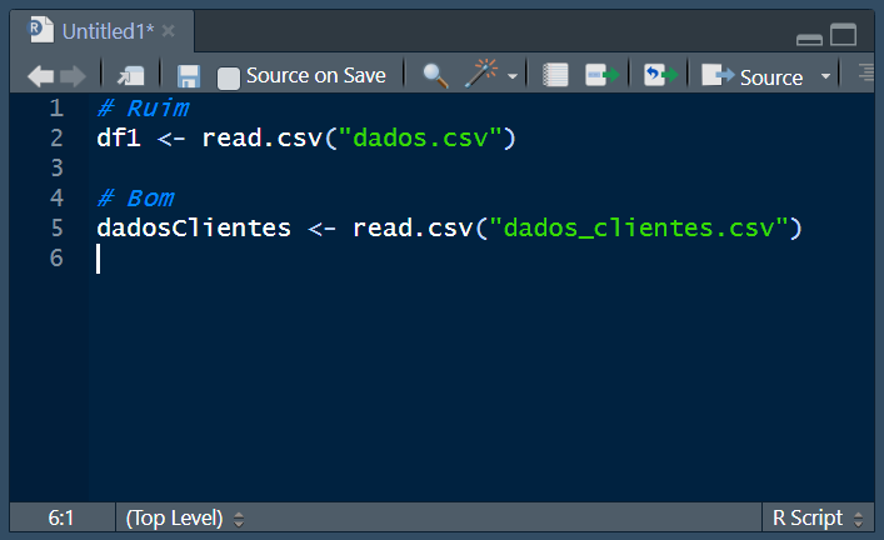
\includegraphics{images/clipboard-2315088477.png}

\subsubsection{Formatação consistente}\label{formatauxe7uxe3o-consistente}

Mantenha um padrão de recuo, espaçamento e formatação. Isso torna o código mais organizado e fácil de ler:

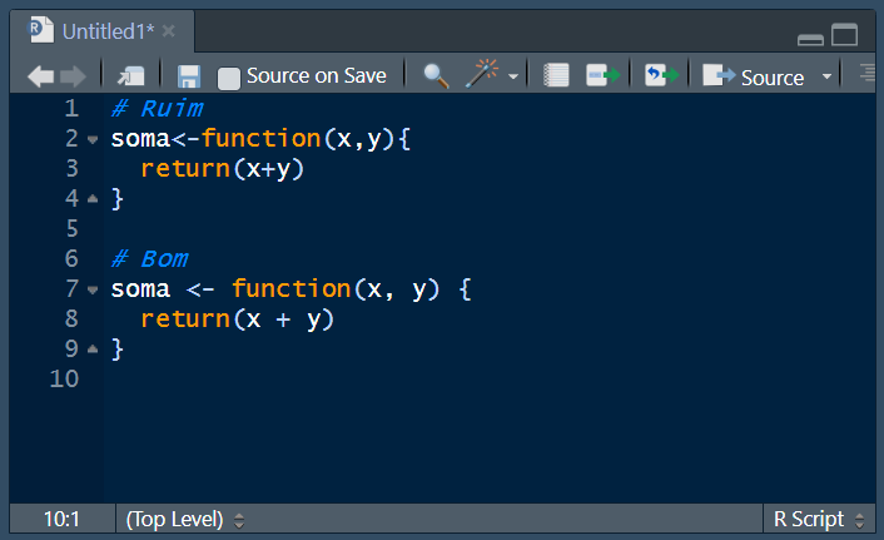
\includegraphics{images/clipboard-2461203963.png}

\subsubsection{Comentários e documentação}\label{comentuxe1rios-e-documentauxe7uxe3o}

Inclua comentários relevantes que expliquem o propósito e a funcionalidade do código. Evite comentários óbvios e mantenha-os atualizados:

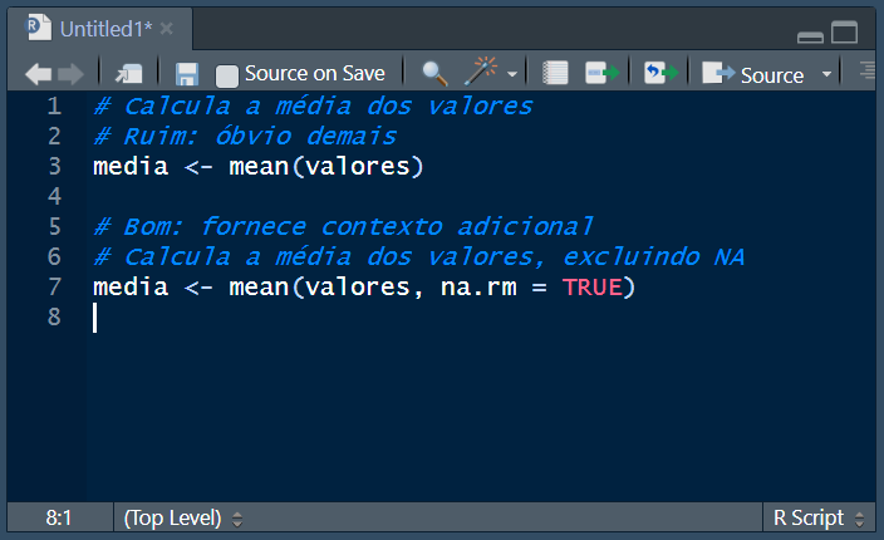
\includegraphics{images/clipboard-978422987.png}

\subsubsection{Simplicidade e modularidade}\label{simplicidade-e-modularidade}

Evite complexidade desnecessária. Divida o código em funções e módulos pequenos e reutilizáveis:

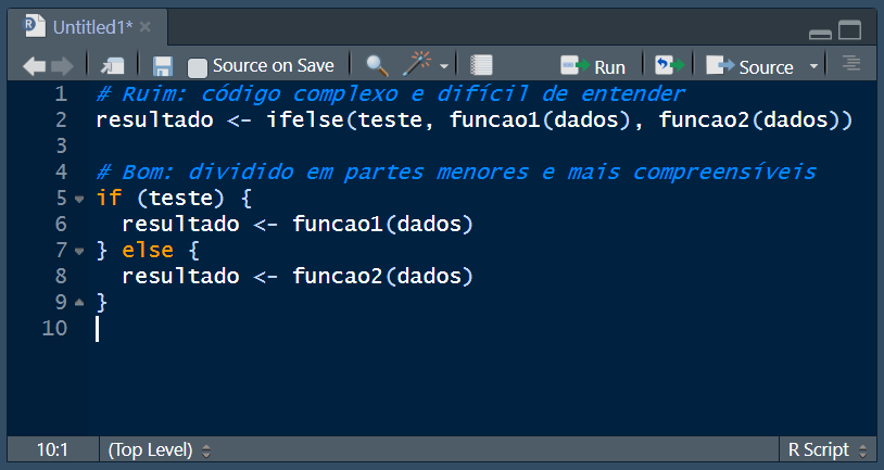
\includegraphics{images/clipboard-1708113605.png}

\subsubsection{Tratamento de erros}\label{tratamento-de-erros}

Manipule e documente adequadamente quaisquer condições de erro para evitar falhas inesperadas:

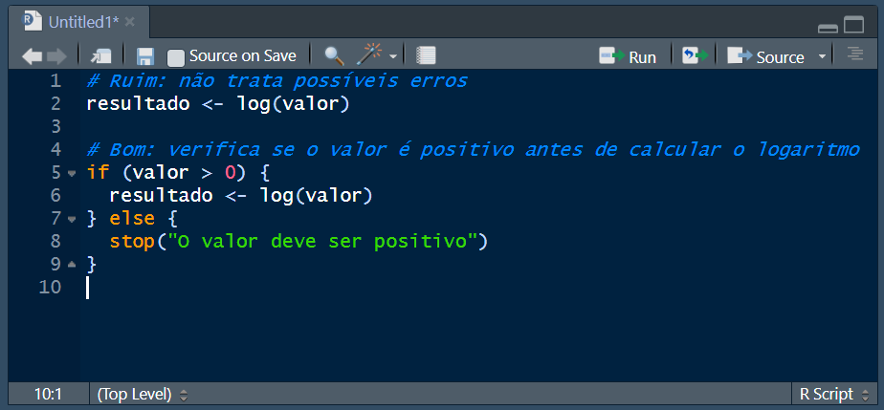
\includegraphics{images/clipboard-2761045831.png}

\subsubsection{Evitar duplicações de código}\label{evitar-duplicauxe7uxf5es-de-cuxf3digo}

Reutilize trechos de código e crie funções ou classes para evitar repetições desnecessárias:

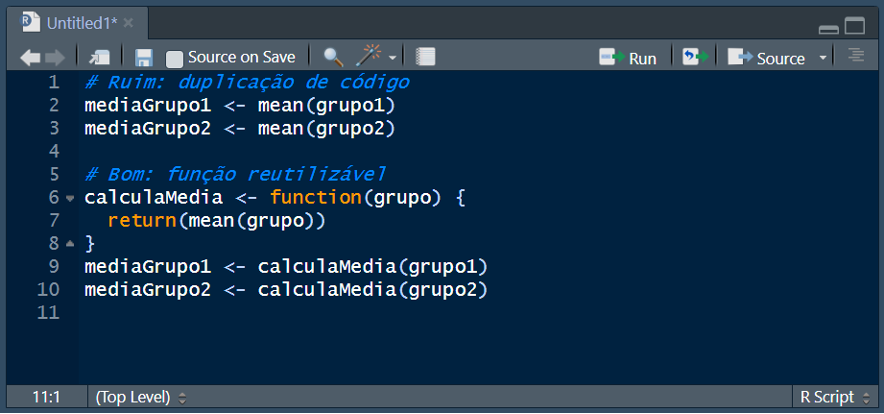
\includegraphics{images/clipboard-491234479.png}

\subsubsection{Vetorização}\label{vetorizauxe7uxe3o}

R é uma linguagem vetorizada, o que significa que muitas operações podem ser realizadas sem o uso explícito de \emph{loops}, tornando o código mais eficiente:

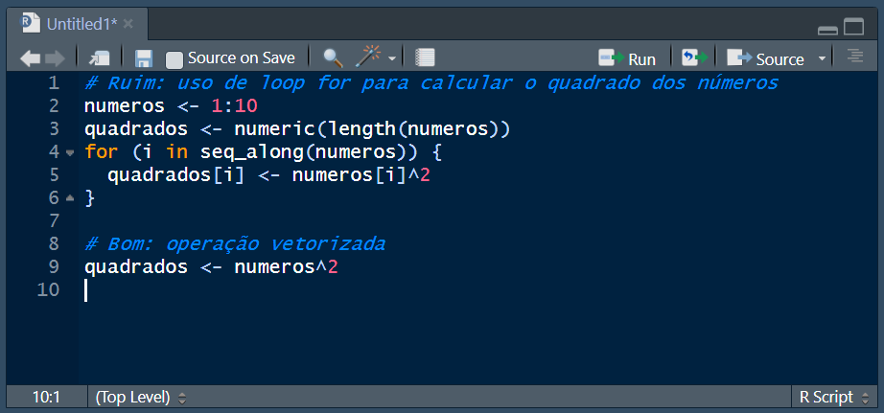
\includegraphics{images/clipboard-2187533748.png}

Seguindo essas práticas, é possível escrever código em R que não apenas atenda aos requisitos funcionais, mas também seja fácil de ler, entender e manter. A chave é sempre buscar a clareza, a simplicidade e a eficiência, facilitando assim o trabalho tanto do autor do código quanto de outros desenvolvedores que possam trabalhar com ele no futuro.

\subsection{Depuração e tratamento de erros em R}\label{depurauxe7uxe3o-e-tratamento-de-erros-em-r}

Escrever código que funcione corretamente é apenas uma parte do desenvolvimento de software; a outra parte é garantir que o código continue funcionando e que possa ser corrigido quando surgirem problemas. A depuração e o tratamento de erros são habilidades essenciais para qualquer programador, e na linguagem R não é diferente. Abaixo estão algumas estratégias e ferramentas para depuração e tratamento de erros em R, acompanhadas de exemplos práticos.

\subsubsection{Depuração interativa}\label{depurauxe7uxe3o-interativa}

A depuração interativa permite que você inspecione o estado do seu programa R enquanto ele está sendo executado. O RStudio oferece ferramentas integradas para isso, como o inspetor de erros e a função `traceback( ) `, que lista a sequência de chamadas que levaram ao erro. Além disso, o RStudio possui ferramentas como ``Rerun with Debug'' e `options(error = browser())`, que abrem uma sessão interativa onde o erro ocorreu.

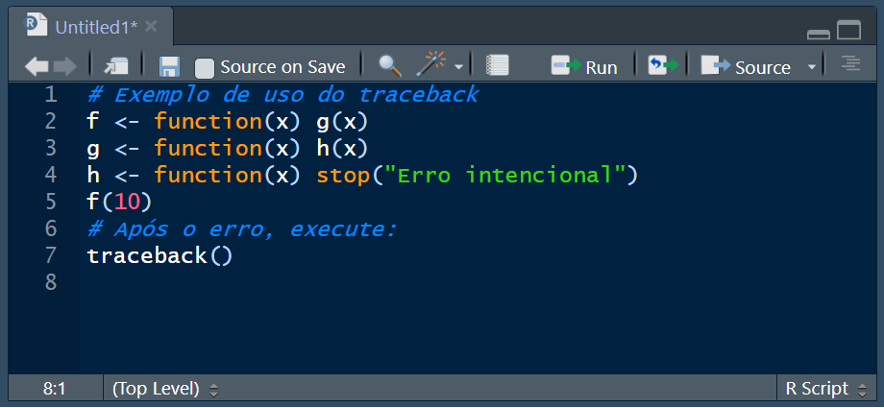
\includegraphics{images/clipboard-3416304030.png}

\subsubsection{Tratamento de erros com tryCatch}\label{tratamento-de-erros-com-trycatch}

A função `tryCatch()` é a principal ferramenta para lidar com erros e avisos em R. Ela permite que você especifique funções manipuladoras que controlam o que acontece quando uma condição é sinalizada.

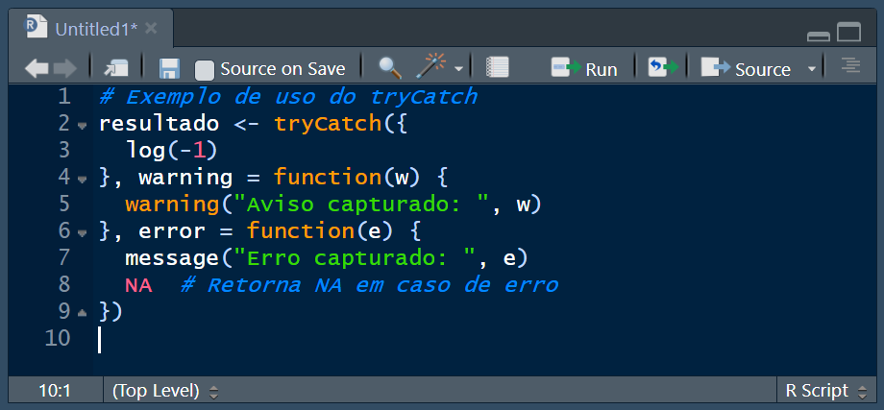
\includegraphics{images/clipboard-3819030973.png}

\subsubsection{Logging de erros}\label{logging-de-erros}

Registrar erros é uma prática padrão no desenvolvimento de software. Em R, você pode usar pacotes de \emph{logging} ou simplesmente registrar erros em um arquivo JSON ou em um banco de dados. Isso é especialmente útil em aplicativos de produção, como aplicativos shiny ou APIs REST.

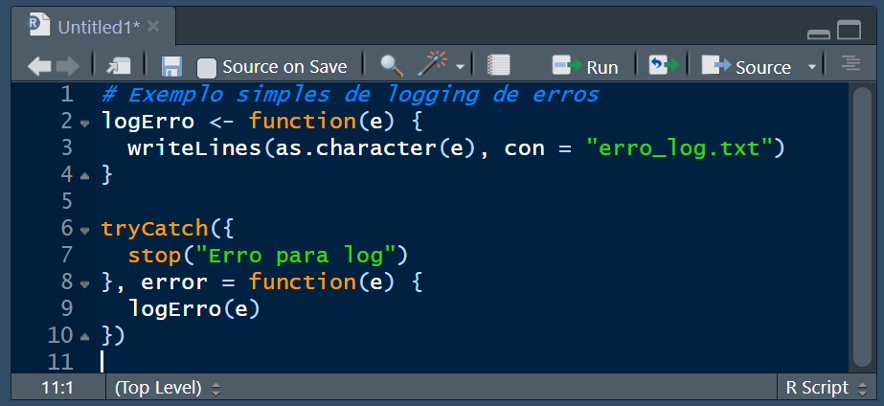
\includegraphics{images/clipboard-2118828263.png}

\subsubsection{Debugging com print}\label{debugging-com-print}

Se as ferramentas de depuração não ajudarem, uma boa alternativa é o ``print debugging'', onde você insere vários comandos `print()` para localizar precisamente o problema e ver os valores das variáveis importantes. É um método lento e primitivo, mas sempre funciona.

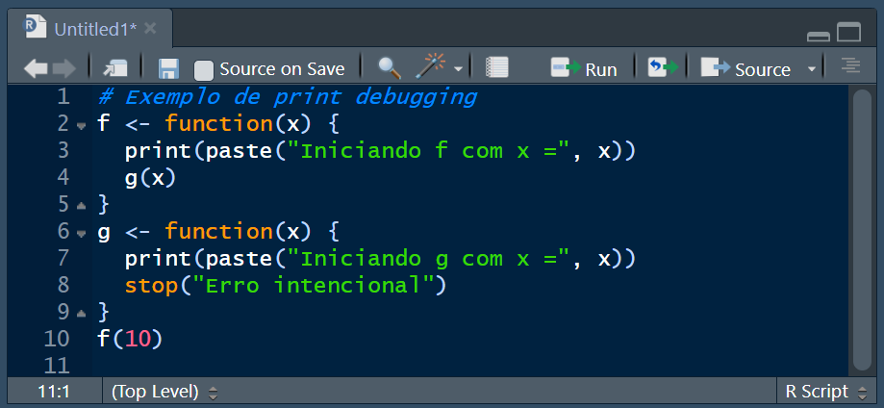
\includegraphics{images/clipboard-2905347804.png}

A depuração e o tratamento de erros são partes cruciais do desenvolvimento em R. Utilizar as ferramentas e estratégias corretas pode economizar tempo e evitar a perda de dados ou resultados importantes. É essencial criar mensagens de erro claras e informativas e documentar o significado dos erros que seu software pode gerar. A experiência e a prática levarão a uma maior maestria na depuração e no tratamento de erros em R.

\subsection{Documentando e compartilhando seu código}\label{documentando-e-compartilhando-seu-cuxf3digo}

Documentar e compartilhar seu código são práticas essenciais para qualquer programador, especialmente para iniciantes em programação que estão aprendendo a linguagem R. Essas práticas não apenas facilitam a colaboração e a revisão por outros, mas também ajudam o próprio autor a entender e manter seu código ao longo do tempo.

\subsubsection{Documentação de código}\label{documentauxe7uxe3o-de-cuxf3digo}

A documentação é a primeira linha de comunicação entre o programador e quem vai ler o código depois, seja o próprio autor em um momento futuro ou outros programadores. Em R, a documentação pode ser feita diretamente no código, usando comentários, e de forma mais estruturada, usando pacotes como o `roxygen2` (\citeproc{ref-wickham2024}{Wickham et al. 2024}), que permite criar uma documentação que pode ser convertida em um manual de ajuda para o pacote.

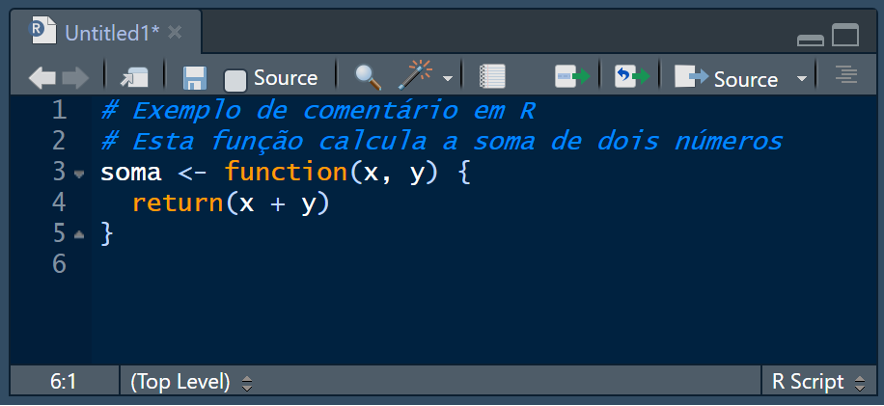
\includegraphics{images/clipboard-3987177554.png}

\subsubsection{Compartilhamento de código}\label{compartilhamento-de-cuxf3digo}

O compartilhamento de código em R pode ser feito de várias maneiras. Uma das mais comuns é através de scripts, que são arquivos de texto com extensão `.R`. Esses scripts podem ser compartilhados por e-mail, repositórios de código como GitHub ou plataformas como \href{https://rpubs.com}{RPubs}, onde é possível publicar análises e códigos para que outros possam ver e usar.

\subsubsection{R Markdown}\label{r-markdown}

Uma ferramenta poderosa para documentar e compartilhar análises em R é o R Markdown (\citeproc{ref-baumer2015}{Baumer and Udwin 2015}). Com ele, é possível combinar texto narrativo com código R que pode ser executado para gerar resultados, que são automaticamente incluídos no documento. Isso é particularmente útil para relatórios, onde a análise e os resultados precisam ser apresentados de forma clara e reproduzível.

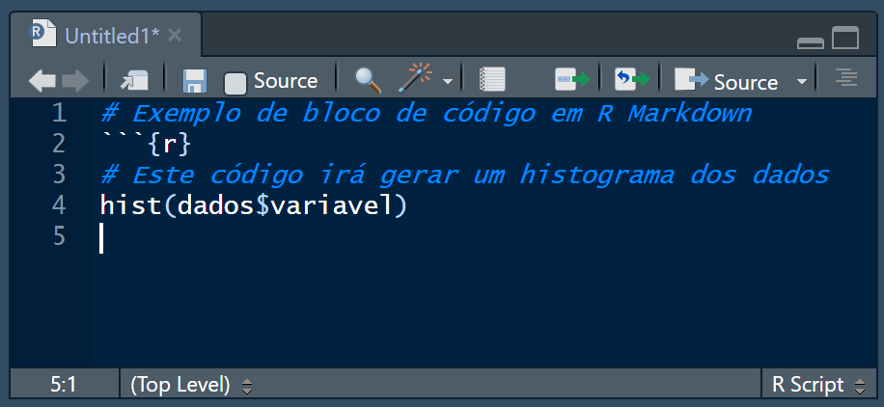
\includegraphics{images/clipboard-1117062658.png}

\subsection{Introdução à análise estatística com R}\label{introduuxe7uxe3o-uxe0-anuxe1lise-estatuxedstica-com-r}

A análise estatística é uma parte fundamental da linguagem de programação R, que foi originalmente desenvolvida com um forte foco em estatística e análise de dados. Aqui está uma introdução detalhada à análise estatística com R.

R é uma linguagem de programação e um ambiente de software para análise estatística e gráficos. Ele fornece uma ampla variedade de técnicas estatísticas, incluindo regressão linear e não linear, análise de séries temporais, classificação, agrupamento e muito mais. Além disso, R é altamente extensível através de pacotes, que são bibliotecas de funções desenvolvidas pela comunidade para estender a funcionalidade do R.

\subsubsection{Estatística Descritiva}\label{estatuxedstica-descritiva}

A estatística descritiva é a primeira etapa na análise de dados. Ela envolve resumir e organizar os dados de maneira que possam ser facilmente compreendidos. As funções básicas do R para estatística descritiva incluem `mean()` para calcular a média, `median()` para a mediana, `sd()` para o desvio padrão, `var()` para a variância, `min()` e `max()` para os valores mínimo e máximo, respectivamente, e `summary()` para obter um resumo estatístico dos dados. As funções mencionadas acima já foram exemplificadas no módulo 2. Tente aplicar essas funções em um novo exemplo (ex.: vet1 \textless- c(1,4,8,3,4,6,7,8,2,6,8,9,2,1,)).

\subsubsection{Visualização de dados}\label{visualizauxe7uxe3o-de-dados}

A visualização de dados é uma parte importante da análise estatística. R fornece várias ferramentas para criar gráficos e visualizações de dados. As funções básicas incluem `plot()` para criar gráficos de dispersão, `hist()` para histogramas, `boxplot()` para boxplots e `barplot()` para gráficos de barras. Além disso, o pacote `ggplot2` oferece uma poderosa e flexível estrutura para criar gráficos complexos. O pacote `ggplot2` será explorado em mais detalhes no próximo módulo.

\textbf{Exemplo}: usando a função ``plot( )''

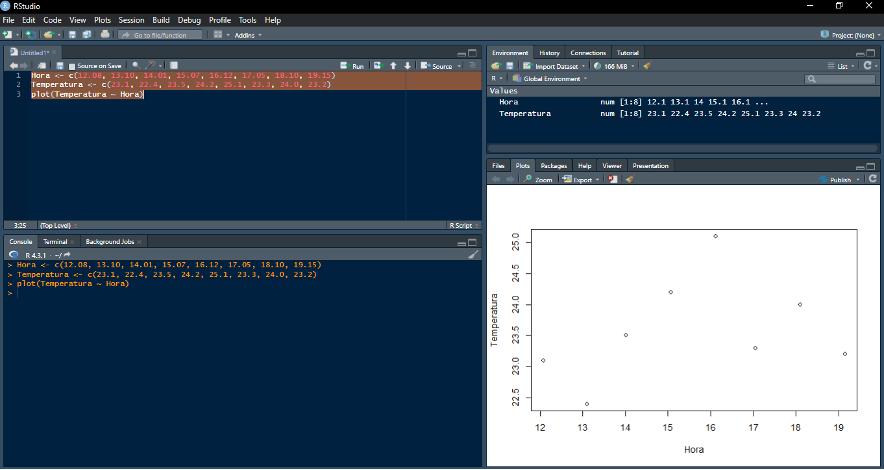
\includegraphics{images/clipboard-3607661657.png}

*Dois vetores, ``Hora'' e ``Temperatura'', foram criados e depois inseridos na função ``plot( )''. Note que a sintaxe da função foi ``plot(Temperatura \textasciitilde{} Hora)'', que é o equivalente de dizer ``Temperatura em função da Hora'' em linguagem R. O mesmo resultado pode ser obtido informando qual vetor ocupa qual eixo: ``plot(x = Hora, y = Temperatura)''.

\textbf{Exemplo}: criando um histograma com a função ``hist( )''

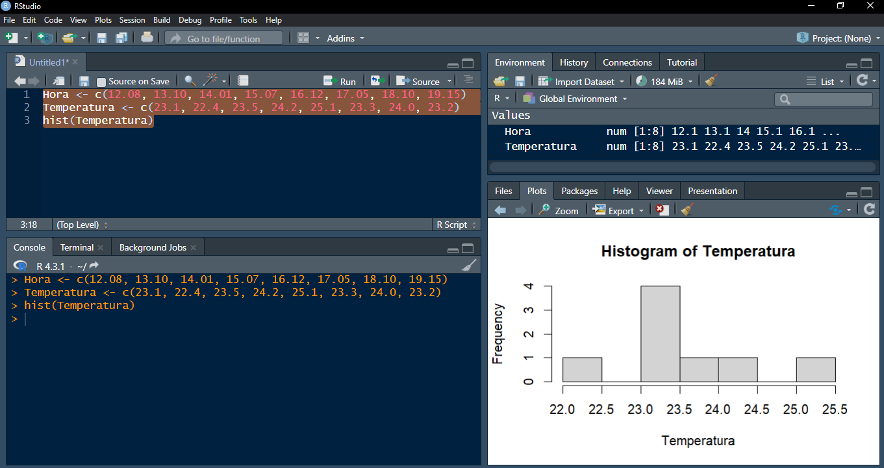
\includegraphics{images/clipboard-680965483.png}

*Utilizando o vetor ``Temperatura'' do exemplo anterior, criou-se um histograma com a função ``hist( )''. Note como temperaturas entre 23,0 e 23,5 ºC são mais comuns do que as outras medidas ao longo do intervalo de tempo avaliado.

\textbf{Exemplo}: criando um boxplot com a função ``boxplot( )''

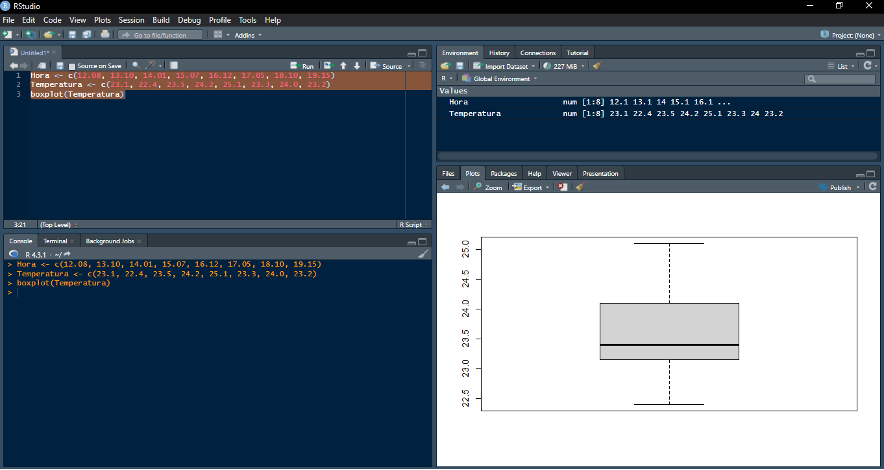
\includegraphics{images/clipboard-1951655399.png}

*Utilizando a mesma estratégia do exemplo anterior, um diagrama de caixa (\emph{boxplot}) foi criado através da função ``boxplot( )''. Se desejar, leia mais sobre \href{https://statplace.com.br/blog/como-interpretar-um-boxplot/}{como interpretar um \emph{boxplot}}, e pratique com novos exercícios.

\subsubsection{Estatística inferencial}\label{estatuxedstica-inferencial}

A estatística inferencial é o processo de usar os dados de uma amostra para inferir propriedades da população. Isso envolve a realização de testes de hipóteses para determinar se um resultado observado é devido ao acaso ou a algum fator subjacente. As funções básicas do R para estatística inferencial incluem `t.test()` para o teste t, `chisq.test()` para o teste do qui-quadrado, `cor.test()` para o teste de correlação, e `lm()` para a regressão linear.

\textbf{Exemplo}: realizando um teste de hipóteses com dois vetores numéricos

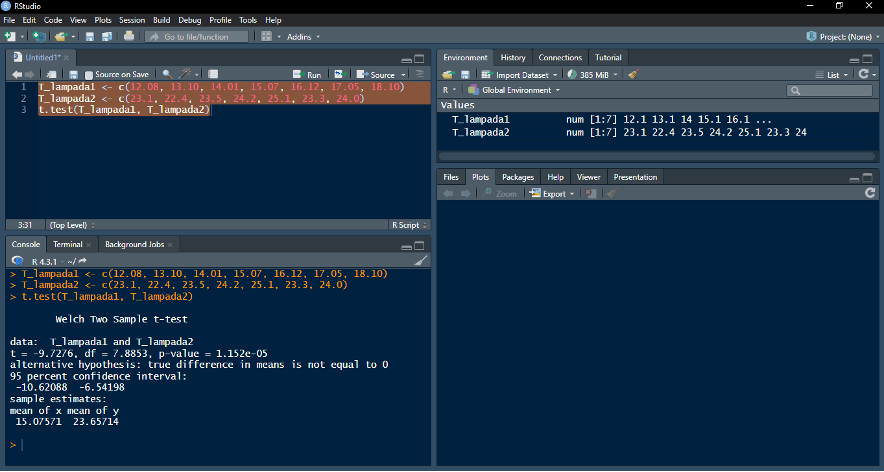
\includegraphics{images/clipboard-2899251105.png}

*Suponhamos que as temperaturas superficiais de duas lâmpadas tenham sido medidas repetidas vezes. Agora, podemos comparar esses vetores numéricos (``T\_lampada1'' e ``T\_lampada2'') considerando a hipótese de que a diferença verdadeira entre as médias de ambos os vetores é igual a 0. Como se observa, a função ``t.test( )'' retorna uma probabilidade muito baixa (\emph{p} = 0.00001152) de que os dois vetores tenham surgido de uma mesma distribuição. Em outras palavras, podemos atribuir confiança razoável de que ambas as lâmpadas possuam temperaturas médias distintas.

\subsubsection{Modelagem estatística}\label{modelagem-estatuxedstica}

A modelagem estatística é o processo de desenvolver um modelo matemático que descreve uma relação entre variáveis. R fornece várias funções para modelagem estatística, incluindo `lm()` para regressão linear, `glm()` para regressão linear generalizada, `anova()` para análise de variância, e `arima()` para modelagem de séries temporais.

\textbf{Exemplo}: avaliando a correlação entre dois vetores numéricos com a função ``lm( )''

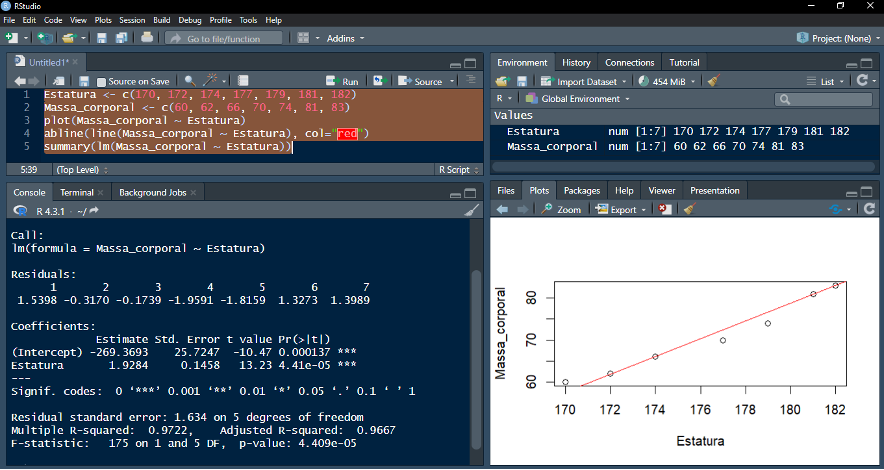
\includegraphics{images/clipboard-870011745.png}

*Dados de estatura e massa corporal de diversas pessoas foram armazenados em vetores numéricos. Um gráfico da relação entre as duas variáveis foi gerado com o código ``plot(Massa\_corporal \textasciitilde{} Estatura)'', seguido da linha vermelha ``abline(line(Massa\_corporal \textasciitilde{} Estatura), col=''red'')''. Como a relação entre estatura e massa corporal parecem proporcionais, a função ``lm( )'' foi utilizada para medir a associação entre os dois vetores. De acordo com o valor de R-quadrado (``\emph{R-squared}'') da função ``summary(lm(Massa\_corporal \textasciitilde{} Estatura))'', 97 \% da variação na massa corporal pode ser explicada pela variação observada na estatura. No exemplo, a função ``summary( )'' é usada para detalhar os resultados do modelo de regressão linear calculado pela função ``lm( )''.

R é uma ferramenta poderosa para análise estatística, oferecendo uma ampla gama de funções para estatística descritiva, visualização de dados, estatística inferencial e modelagem estatística. Aprender a usar R para análise estatística pode abrir novas oportunidades para a exploração e compreensão de dados.

\subsection{Usando R para estatísticas descritivas}\label{usando-r-para-estatuxedsticas-descritivas}

A linguagem de programação R é uma ferramenta poderosa para a realização de estatísticas descritivas, que são métodos utilizados para resumir e organizar um conjunto de dados de maneira que possam ser facilmente compreendidos. Abaixo, você encontrará uma explanação detalhada de como usar R para estatísticas descritivas. Exemplos dessas funções podem ser encontradas no módulo 2, mas é recomendado que você pratique os códigos deste módulo em seu ambiente RStudio.

\subsubsection{Medidas de tendência central}\label{medidas-de-tenduxeancia-central-1}

As medidas de tendência central são estatísticas que indicam onde os dados estão centrados. As principais medidas de tendência central são a média, a mediana e a moda.

\begin{enumerate}
\def\labelenumi{\arabic{enumi}.}
\item
  \textbf{Média}: a média de um conjunto de dados é calculada somando todos os valores e dividindo pelo número de valores. No R, a média é calculada usando a função `mean()`. Por exemplo, `mean(c(1, 2, 3, 4, 5))` calcula a média do vetor de números de 1 a 5.
\item
  \textbf{Mediana}: a mediana é o valor que divide os dados ao meio quando estão ordenados. No R, a mediana é calculada usando a função `median()`. Por exemplo, `median(c(1, 2, 3, 4, 5))` calcula a mediana do vetor de números de 1 a 5.
\item
  \textbf{Moda}: a moda é o valor mais frequente em um conjunto de dados. R não tem uma função embutida para calcular a moda, mas pode ser calculada usando funções de outros pacotes ou escrevendo sua própria função.
\end{enumerate}

\subsubsection{Medidas de dispersão}\label{medidas-de-dispersuxe3o-1}

As medidas de dispersão são estatísticas que indicam o quanto os dados estão espalhados. As principais medidas de dispersão são a variância, o desvio padrão e a amplitude.

\begin{enumerate}
\def\labelenumi{\arabic{enumi}.}
\item
  \textbf{Variância}: a variância é uma medida da dispersão que indica o quanto os valores se desviam da média. No R, a variância é calculada usando a função `var()`. Por exemplo, `var(c(1, 2, 3, 4, 5))` calcula a variância do vetor de números de 1 a 5.
\item
  \textbf{Desvio padrão}: o desvio padrão é a raiz quadrada da variância e fornece uma medida de dispersão que está na mesma unidade que os dados. No R, o desvio padrão é calculado usando a função `sd()`. Por exemplo, `sd(c(1, 2, 3, 4, 5))` calcula o desvio padrão do vetor de números de 1 a 5.
\item
  \textbf{Amplitude}: a amplitude é a diferença entre o maior e o menor valor em um conjunto de dados. No R, a amplitude pode ser calculada subtraindo o resultado da função `min()` do resultado da função `max()`. Por exemplo, `max(c(1, 2, 3, 4, 5)) - min(c(1, 2, 3, 4, 5))` calcula a amplitude do vetor de números de 1 a 5.
\end{enumerate}

\subsubsection{Resumo dos dados}\label{resumo-dos-dados}

A função `summary()` no R fornece um resumo estatístico dos dados, incluindo a média, a mediana, o mínimo, o máximo, o primeiro quartil e o terceiro quartil. Por exemplo, `summary(c(1, 2, 3, 4, 5))` fornece um resumo do vetor de números de 1 a 5.

R é uma ferramenta poderosa para estatísticas descritivas, oferecendo uma ampla gama de funções para calcular medidas de tendência central, medidas de dispersão e resumos de dados. Aprender a usar R para estatísticas descritivas pode abrir novas oportunidades para a exploração e compreensão de dados.

\subsection{Estatísticas inferenciais com R}\label{estatuxedsticas-inferenciais-com-r}

As estatísticas inferenciais com R envolvem o uso de técnicas estatísticas para fazer generalizações sobre uma população com base em uma amostra de dados. Essas técnicas são fundamentais para a tomada de decisões baseada em dados e para a pesquisa científica.

\subsubsection{Conceitos básicos}\label{conceitos-buxe1sicos}

Antes de realizar a inferência estatística, é importante entender alguns conceitos básicos, como população, amostra, parâmetro e estimativa. A população é o conjunto completo de observações que estão sendo estudadas, enquanto uma amostra é um subconjunto dessa população. Um parâmetro é uma medida resumida da população, como a média populacional, e uma estimativa é o correspondente calculado a partir da amostra.

\subsubsection{Testes de hipóteses}\label{testes-de-hipuxf3teses-1}

Um dos pilares da inferência estatística é o teste de hipóteses. O objetivo é testar uma afirmação (hipótese) sobre um parâmetro populacional. No R, funções como `t.test()`, `chisq.test()` e `anova()` são usadas para realizar diferentes tipos de testes de hipóteses.

Por exemplo, o `t.test()` é usado para comparar as médias de duas amostras e determinar se elas são significativamente diferentes. O teste do qui-quadrado (`chisq.test()`) é frequentemente usado para testar a independência entre duas variáveis categóricas. A análise de variância (ANOVA), realizada através da função `anova()`, é usada para comparar as médias de três ou mais grupos.

\subsubsection{Intervalos de confiança}\label{intervalos-de-confianuxe7a}

Outra ferramenta importante na inferência estatística é o intervalo de confiança, que fornece um intervalo estimado dentro do qual é provável que o parâmetro populacional esteja. No R, o `t.test()` e outras funções de teste fornecem intervalos de confiança como parte de seus resultados.

\subsubsection{Regressão e correlação}\label{regressuxe3o-e-correlauxe7uxe3o}

A análise de regressão é usada para entender a relação entre variáveis. No R, a função `lm()` é usada para realizar regressão linear, que modela a relação entre uma variável dependente e uma ou mais variáveis independentes. A correlação, que mede a força e a direção da relação linear entre duas variáveis, pode ser calculada com a função `cor()`.

\subsubsection{Análise de séries temporais}\label{anuxe1lise-de-suxe9ries-temporais}

A análise de séries temporais é um tipo de inferência estatística que lida com dados coletados ao longo do tempo. No R, funções como `ts()` para criar objetos de séries temporais e `arima()` para modelagem de séries temporais são usadas para analisar como os dados mudam ao longo do tempo.

\textbf{Exemplo}: utilizando a função ``arima( )'' para prever uma série temporal

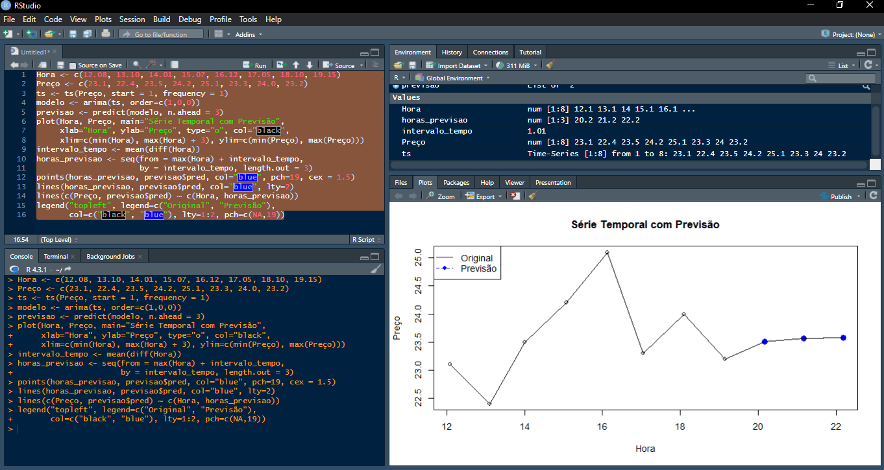
\includegraphics{images/clipboard-3461101962.png}

*Utilizando os dados de tempo e variação do preço de uma determinada ação, podemos aplicar a função ``arima( )'' para criar um modelo e prever a variação de preço para as próximas 3 horas. Veja como o gráfico representa a série temporal original seguida de três pontos (azuis) informando a variação futura prevista.

A inferência estatística no R é uma área vasta e complexa, que requer um entendimento sólido de teoria estatística e a habilidade de aplicar essa teoria usando o R. As funções e pacotes disponíveis no R tornam a linguagem uma ferramenta poderosa para realizar análises inferenciais e extrair insights significativos de dados amostrais.

\subsection{Fundamentos da visualização de dados em R}\label{fundamentos-da-visualizauxe7uxe3o-de-dados-em-r}

A visualização é uma etapa crucial na análise de dados, pois permite aos analistas e cientistas de dados entender e interpretar os dados de maneira eficaz, além de comunicar suas descobertas de forma clara. No R, uma linguagem de programação amplamente utilizada para estatística e análise de dados, existem várias ferramentas e pacotes dedicados à visualização de dados. Aqui está uma explanação detalhada sobre os fundamentos da visualização de dados em R.

\subsubsection{Gráficos base do R}\label{gruxe1ficos-base-do-r}

O R possui um sistema de gráficos base que permite a criação de uma ampla variedade de gráficos, incluindo gráficos de linhas, barras, histogramas, boxplots, e scatter plots. Esses gráficos são gerados usando funções simples, como `plot()`, `hist()`, `barplot()`, e `boxplot()`. Por exemplo, a função `plot()` pode ser usada para criar gráficos de dispersão ou linhas, dependendo dos argumentos fornecidos. A função `hist()` é usada para criar histogramas, que são úteis para visualizar a distribuição de uma única variável numérica. Veja, abaixo, uma lista de gráficos comuns em \emph{Base R}:

\begin{enumerate}
\def\labelenumi{\arabic{enumi}.}
\item
  \textbf{Gráficos de dispersão (scatter plots)}: utilizados para visualizar a relação entre duas variáveis numéricas. A função `plot()` é a mais comum para criar esses gráficos.
\item
  \textbf{Histogramas}: usados para representar a distribuição de uma única variável numérica. A função `hist()` é utilizada para gerar histogramas.
\item
  \textbf{Gráficos de linhas}: úteis para visualizar dados ao longo do tempo ou sequências ordenadas. A função `plot()` também pode ser usada para criar gráficos de linhas, alterando o tipo de ponto para uma linha.
\item
  \textbf{Gráficos de barras}: permitem comparar quantidades entre diferentes grupos. As funções `barplot()` ou `hist()` podem ser usadas para criar gráficos de barras.
\item
  \textbf{Boxplots}: fornecem uma representação visual da distribuição de uma variável numérica, destacando a mediana, os quartis e os valores discrepantes. A função `boxplot()` é usada para criar boxplots.
\end{enumerate}

Vamos praticar um exemplo da função ``barplot( )''.

\textbf{Exemplo}: criando um gráfico de barras com a função ``barplot( )''

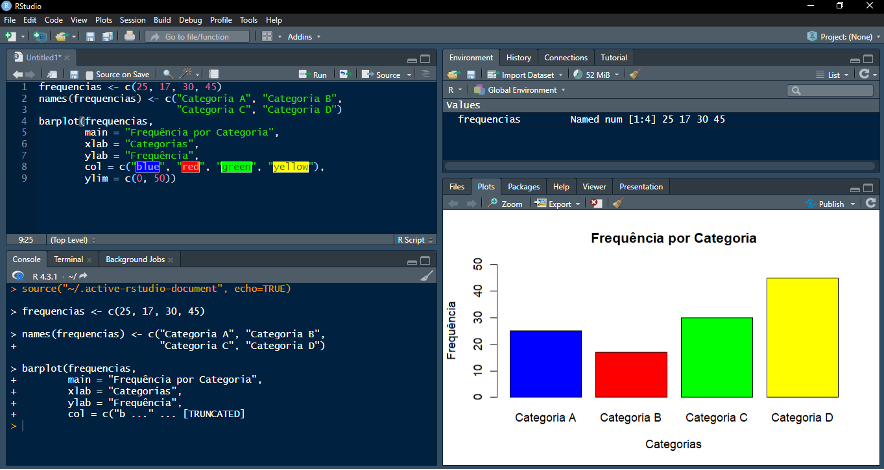
\includegraphics{images/clipboard-18805364.png}

*Considerando um vetor contendo a contagem de frequências para quatro categorias distintas (Categorias A, B, C e D), um gráfico de barras pode ser gerado com a função ``barplot( )''. Também é possível personalizar diversos aspectos do gráfico dentro da função: ``main'' = título do gráfico; ``xlab'' = título do eixo x; ``ylab'' = título do eixo y; ``col'' = cor de preenchimento das barras; ``ylim'' = limites numéricos do eixo y.

\subsubsection{Personalização de gráficos}\label{personalizauxe7uxe3o-de-gruxe1ficos}

Os gráficos base do R são altamente personalizáveis. Você pode modificar títulos, rótulos dos eixos, cores, tipos de linhas e pontos, e muito mais, usando argumentos adicionais nas funções de plotagem. Por exemplo, você pode usar o argumento `main` para adicionar um título ao gráfico, `xlab` e `ylab` para rótulos dos eixos X e Y, respectivamente, e `col` para alterar a cor dos pontos ou linhas.

Também é possível sobrepor elementos gráficos em R base. Por exemplo, você pode gerar uma linha que conecta todos os pontos em um gráfico de dispersão (``plot( )'' + ``lines( )''), ou até mesmo adicionar uma legenda para diferentes barras (``barplot( )'' + ``legend( )'').

\textbf{Exemplo}: sobrepondo elementos gráficos em R base

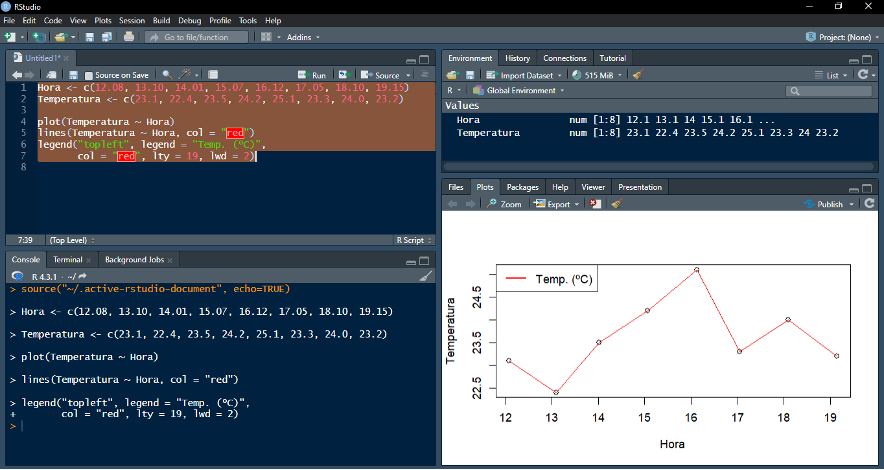
\includegraphics{images/clipboard-2859898208.png}

*No exemplo acima, um gráfico de dispersão foi criado utilizando a função ``plot( )''. Logo abaixo, uma função ``lines( )'' cria uma linha vermelha que conecta todos os pontos do gráfico. Finalmente, a função ``legend( )'' permite a criação de uma legenda para os dados.

\subsubsection{O pacote ggplot2}\label{o-pacote-ggplot2}

Além do sistema de gráficos base, o R oferece o pacote `ggplot2` (lembre-se que pacotes devem ser instalados no primeiro uso e importados sempre que utilizados em uma nova sessão), que é baseado nos princípios da ``Gramática dos Gráficos''. O `ggplot2` permite a construção de gráficos complexos de maneira incremental, adicionando camadas de elementos gráficos. Um gráfico no `ggplot2` começa com a função `ggplot()`, à qual são adicionadas camadas usando o operador `+`. Por exemplo, você pode começar definindo os dados e as estéticas (`aes`) e, em seguida, adicionar uma camada para o tipo de gráfico (como `geom\_point()` para um scatter plot ou `geom\_histogram()` para um histograma).

\textbf{Exemplo}: criando um gráfico básico com a função ``ggplot( )''

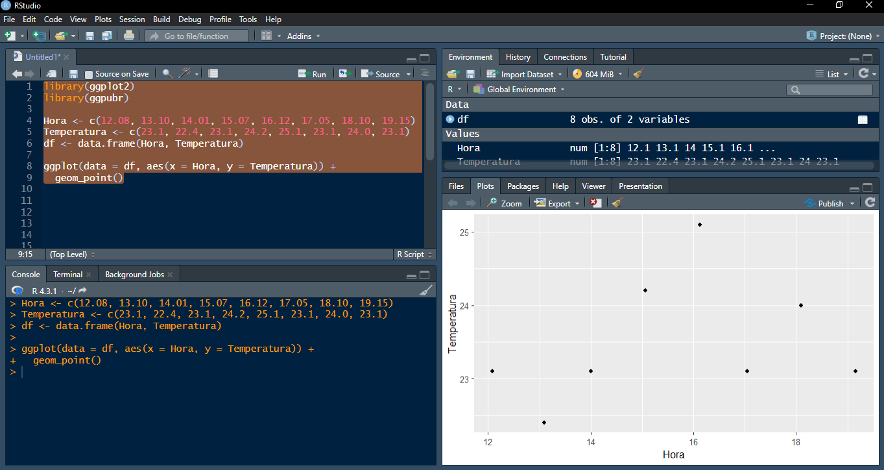
\includegraphics{images/clipboard-1758074744.png}

*Primeiro, os pacotes desejados foram importados para o ambiente R. No caso do exemplo acima, ``ggplot2'' é o pacote necessário para gerar gráficos, enquanto ``ggpubr'' será utilizado para manipular a apresentação do gráfico no próximo exemplo. Antes de criar o gráfico, um data frame (``df'') foi gerado a partir dos vetores ``Hora'' e ``Temperatura''. Depois, um objeto ggplot é criado utilizando a função ``ggplot(data = df, aes(x = Hora, y = Temperatura))''; para adicionar os pontos ao gráfico, porém, é necessário adicionar um ``+'' ao lado da função e, em seguida, informar a função para o tipo de gráfico. No caso do exemplo, a função ``geom\_point( )'' cria um gráfico de dispersão simples.

Múltiplos gráficos `ggplot` podem ser organizados em uma mesma figura. Uma forma de fazê-lo é com o pacote `ggpubr`. A função `ggarrange()` no R é uma ferramenta flexível do pacote `ggpubr` que permite organizar múltiplos gráficos `ggplot` em uma única página, com a capacidade de especificar o número de colunas e linhas, bem como criar uma legenda comum para vários gráficos.

Por exemplo, se você tiver três gráficos diferentes armazenados nas variáveis `bxp`, `dp` e `dens`, você pode organizá-los em uma grade de 2 colunas e 2 linhas usando `ggarrange(bxp, dp, dens, ncol = 2, nrow = 2)`. Além disso, se você deseja usar uma legenda comum para múltiplos gráficos que compartilham as mesmas estéticas, como cor ou forma, você pode fazer isso com `ggarrange(bxp, dp, common.legend = TRUE)`, onde `bxp` e `dp` são dois gráficos que você deseja combinar. Isso é particularmente útil quando você tem várias visualizações dos mesmos dados e quer evitar a repetição de legendas, tornando o resultado mais limpo e fácil de ler.

\textbf{Exemplo}: organizando mais de um gráfico por tela com ``ggarrange( )''

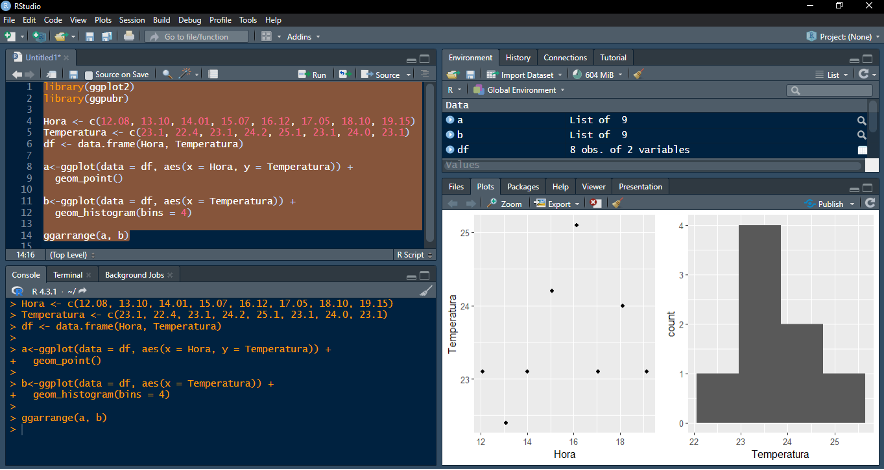
\includegraphics{images/clipboard-469555772.png}

*Utilizando uma continuação do exemplo anterior, um novo gráfico foi criado (``geom\_histogram( )''). Depois, atribuiu-se o primeiro gráfico à variável ``a'' e o segundo à variável ``b''. Finalmente, bastou informar à função ``ggarrage( )'' quais gráficos devem ser organizados no mesmo plano. Tente inverter a ordem dos objetos na função ``ggarrange'' (ex.: ``ggarrange(b, a)'').

\subsubsection{Visualização de dados multivariados}\label{visualizauxe7uxe3o-de-dados-multivariados}

Tanto o sistema de gráficos base quanto o `ggplot2` oferecem opções para visualizar dados multivariados. Por exemplo, você pode usar cores, formas ou tamanhos de pontos para representar variáveis adicionais em um scatter plot. No `ggplot2`, isso é feito especificando estéticas adicionais dentro da função `aes()`.

A facetação é uma técnica poderosa no `ggplot2` que permite dividir os dados em subconjuntos e plotar cada subconjunto em seu próprio painel dentro do gráfico. Isso é útil para comparar subgrupos de dados. A facetação pode ser realizada usando as funções `facet\_wrap()` ou `facet\_grid()`.

\textbf{Exemplo}: utilizando ``facet\_grid( )'' para facetar um gráfico em seus segmentos

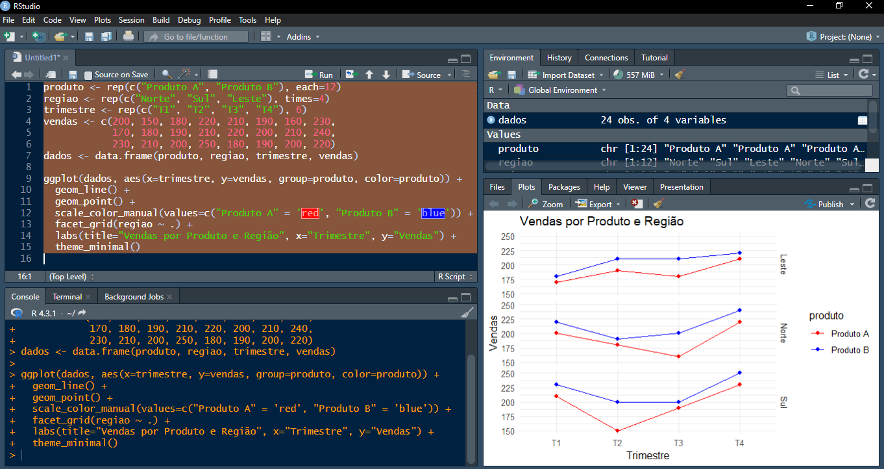
\includegraphics{images/clipboard-928999128.png}

*O código do exemplo acima cria um conjunto de dados e um gráfico correspondente. Primeiramente, são criadas quatro variáveis: `produto`, que repete os nomes ``Produto A'' e ``Produto B'' doze vezes cada; `regiao`, que repete os nomes ``Norte'', ``Sul'' e ``Leste'' quatro vezes cada; `trimestre`, que repete os trimestres ``T1'', ``T2'', ``T3'' e ``T4'' seis vezes; e `vendas`, que contém uma série de valores representando as vendas. Essas variáveis são combinadas em um `data.frame` chamado `dados`. Em seguida, utiliza-se o ggplot2 para criar um gráfico de linhas com pontos, onde o eixo x representa os trimestres, o eixo y as vendas, as linhas e pontos são agrupados e coloridos de acordo com o produto, e o gráfico é dividido em painéis por região utilizando a função ``facet\_grid( )''. Além disso, são definidas cores manuais para os produtos, adicionados títulos aos eixos e ao gráfico, e aplicado um tema minimalista.

\subsubsection{Extensões do ggplot2}\label{extensuxf5es-do-ggplot2}

Existem vários pacotes que estendem as capacidades do `ggplot2`, adicionando novos tipos de gráficos ou funcionalidades. Por exemplo, o pacote `ggplotly` permite converter gráficos `ggplot2` em gráficos interativos, e o `gganimate` permite criar animações a partir de gráficos `ggplot2`.

\textbf{Exemplo}: criando um gráfico interativo a partir de um ggplot com ``ggplotly( )''

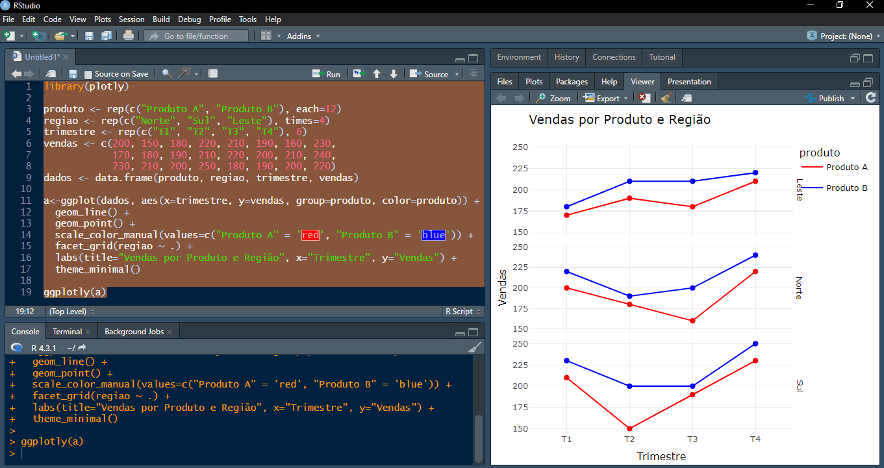
\includegraphics{images/clipboard-465180566.png}

*Baseado no código do exemplo anterior, foi possível elaborar um gráfico interativo em três simples passos: 1. Importar o pacote ``plotly'' utilizando ``library(plotly)''; 2. Atribuir o ggplot previamente criado a uma variável ``a'' (basta inserir ``a \textless- `` logo antes do início do código para o gráfico; 3. Fornecer o objeto ``a'' à função ``ggplotly( )''. O gráfico gerado, apesar de similar ao anterior, se torna interativo e permite funções como zoom, salvar como figura, etiqueta dinâmica de dados e outras.

A visualização de dados em R é uma área rica e flexível, com muitas opções disponíveis para o analista. Seja usando o sistema de gráficos base para gráficos simples e rápidos ou explorando a profundidade e flexibilidade do `ggplot2` para gráficos mais complexos e polidos, o R oferece ferramentas poderosas para transformar dados brutos em insights visuais compreensíveis.

\subsubsection{Visualização de dados geoespaciais}\label{visualizauxe7uxe3o-de-dados-geoespaciais}

A visualização de dados geoespaciais é outra técnica avançada que pode ser realizada em R, utilizando pacotes como `ggplot2` em conjunto com `sf` (\citeproc{ref-pebesma2024}{Pebesma et al. 2024}) para criar mapas detalhados. Esses mapas podem representar desde a distribuição geográfica de eventos até análises espaciais complexas, como clusters ou padrões de movimento.

\textbf{Exemplo}: criando um mapa a partir de dados geoespaciais com o pacote ``sf''

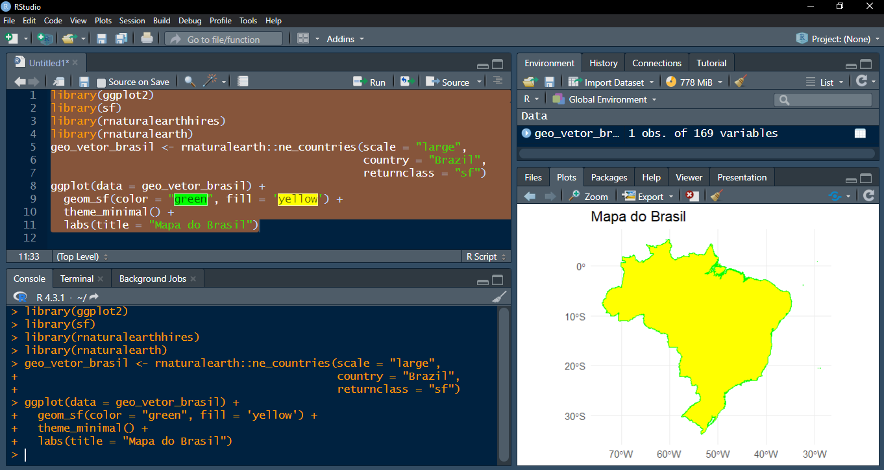
\includegraphics{images/clipboard-3449562011.png}

*O código do exemplo acima utiliza as bibliotecas `ggplot2`, `sf` e `rnaturalearth` para criar um mapa do Brasil. A função `ne\_countries` do pacote `rnaturalearth` é usada para obter os dados geográficos do Brasil, especificando que queremos os dados em uma escala grande e que o formato de retorno seja um objeto `sf`, que é um padrão para trabalhar com dados espaciais no R. O objeto `geo\_vetor\_brasil` contém esses dados e é passado para a função `ggplot`, que inicia a construção do gráfico. A função `geom\_sf` é utilizada para adicionar os dados espaciais ao gráfico, com a cor das linhas definida como verde e o preenchimento como amarelo, representando as fronteiras e o interior do país, respectivamente. O tema `theme\_minimal` é aplicado para um visual limpo e a função `labs` adiciona um título ao gráfico. O resultado é um mapa do Brasil com fronteiras destacadas em verde e interior em amarelo.

\subsubsection{Animações com gganimate}\label{animauxe7uxf5es-com-gganimate}

O pacote `gganimate` (\citeproc{ref-pedersen2024}{Pedersen et al. 2024}) estende as capacidades do `ggplot2`, permitindo criar animações a partir de gráficos. Isso pode ser particularmente útil para visualizar mudanças nos dados ao longo do tempo, como tendências econômicas, padrões climáticos ou o progresso de uma epidemia.

\textbf{Exemplo}: criando um gráfico animado com o pacote ``gganimate''

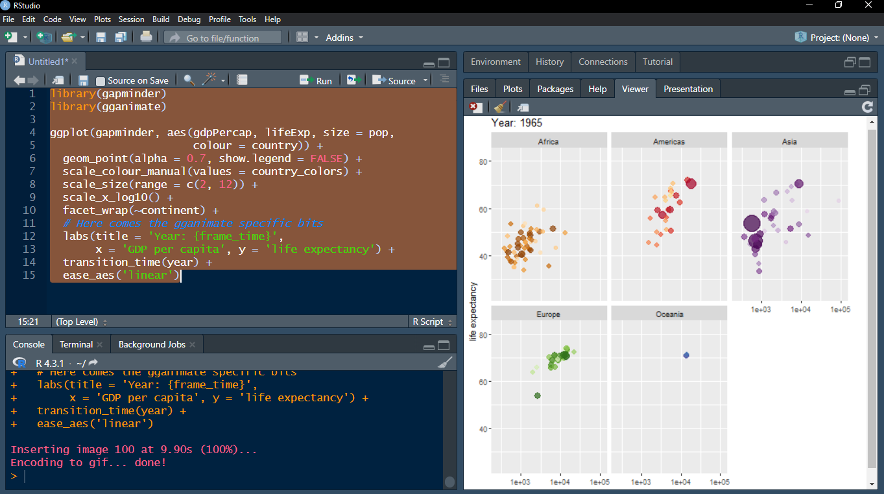
\includegraphics{images/clipboard-342580043.png}

*No exemplo acima, foram utilizadas as bibliotecas `gapminder`(\citeproc{ref-bryan2023}{Bryan 2023}) e `gganimate` para criar uma animação que mostra a relação entre o PIB per capita (GDP per capita), a expectativa de vida (life expectancy) e o tamanho da população (pop) de diferentes países ao longo do tempo. A função `ggplot` inicia a construção do gráfico com os dados do `gapminder`, e a função `aes` define as variáveis para os eixos x e y, o tamanho dos pontos e a cor de acordo com o país. `geom\_point` adiciona pontos ao gráfico com uma transparência de 0.7 e sem legenda. `scale\_colour\_manual` permite a personalização das cores dos pontos por país, enquanto `scale\_size` ajusta o intervalo de tamanho dos pontos. `scale\_x\_log10` transforma o eixo x em uma escala logarítmica para melhor visualização dos dados. `facet\_wrap` divide o gráfico por continente. As funções específicas do `gganimate`, como `transition\_time` e `ease\_aes`, são usadas para criar a animação ao longo do tempo, definida pela variável `year`, e para suavizar a transição entre os frames. O título do gráfico é atualizado dinamicamente para mostrar o ano correspondente a cada frame da animação. Veja a animação \href{https://gganimate.com/reference/figures/README-unnamed-chunk-4-1.gif}{clicando aqui}.

\subsubsection{Dashboards interativos com Shiny}\label{dashboards-interativos-com-shiny}

O pacote `shiny` (\citeproc{ref-chang2024}{Chang et al. 2024}) permite criar aplicativos web interativos diretamente em R. Esses dashboards podem incluir uma variedade de elementos de entrada e saída, permitindo aos usuários interagir com os dados e visualizações em tempo real. Shiny é uma ferramenta poderosa para a construção de ferramentas analíticas interativas e personalizadas.

\textbf{Exemplo}: aplicação shiny para metanálises criada em RStudio

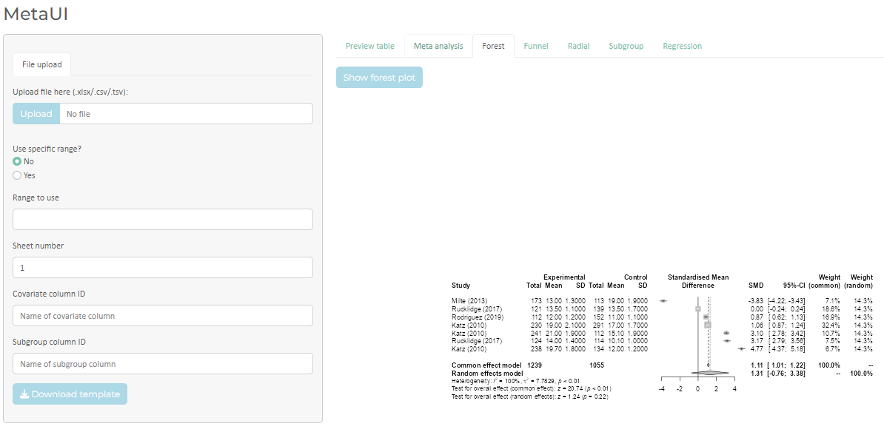
\includegraphics{images/clipboard-3316300773.png}

*A produção de aplicações e \emph{dashboards shiny} é um processo mais complexo do que os exemplos vistos anteriormente. Sua utilização, porém, permite a criação de ferramentas especializadas para pesquisa, trabalho e negócios. Depois de criadas, essas aplicações podem poupar muitas horas de trabalho de um analista ou até mesmo permitir que pessoas sem o conhecimento de programação possam realizar as análises necessárias.

\subsubsection{Tabelas e quadros em R}\label{tabelas-e-quadros-em-r}

Para criar tabelas no R, podemos usar a função `table()` para tabular dados e a função `View()` para visualizar data frames em formato de tabela. Uma forma de visualizar seus dados sem a utilização da função ``View( )'' é clicar no ícone de uma tabela ou uma lupa:


\includegraphics{images/clipboard-4018646742.png}

que aparecem na aba ``Environment'' da janela superior direita. Além disso, o pacote `knitr` (\citeproc{ref-xieaut2024}{Xie {[}aut et al. 2024}) oferece a função `kable()`, que cria tabelas formatadas para relatórios e documentos.

\textbf{Exemplo}: criando uma tabela com a função ``kable( )''

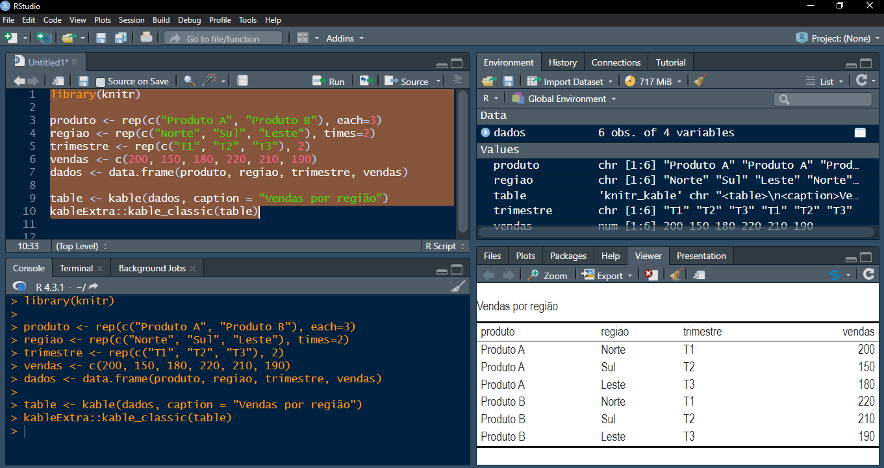
\includegraphics{images/clipboard-2208731083.png}

*Utilizando dados modificados do exemplo anterior, uma tabela kable foi criada. Primeiro, o pacote ``knitr'' foi importado para o ambiente. Em seguida, criou-se um objeto ``table'' com a função ``kable( )'' que recebeu o data frame ``dados''. Finalmente, fornecendo o objeto ``table'' à função ``kable\_classic( )'' (não é necessário utilizar ``kableExtra::'' antes da função), foi possível criar uma tabela.

\section{Python para análise estatística}\label{python-para-anuxe1lise-estatuxedstica}

\section{Visualização de dados e figuras científicas}\label{visualizauxe7uxe3o-de-dados-e-figuras-cientuxedficas}

\chapter{Comunicação científica}\label{comunicauxe7uxe3o-cientuxedfica}

\section{Redação de artigos científicos}\label{redauxe7uxe3o-de-artigos-cientuxedficos}

\section{Estrutura de relatórios de pesquisa}\label{estrutura-de-relatuxf3rios-de-pesquisa}

\section{Apresentações orais e posters}\label{apresentauxe7uxf5es-orais-e-posters}

\section{Publicação e revisão por pares}\label{publicauxe7uxe3o-e-revisuxe3o-por-pares}

\chapter{Ética e boas práticas em pesquisa}\label{uxe9tica-e-boas-pruxe1ticas-em-pesquisa}

\section{Consentimento informado e conformidade ética}\label{consentimento-informado-e-conformidade-uxe9tica}

\section{Plágio e integridade acadêmica}\label{pluxe1gio-e-integridade-acaduxeamica}

\section{Regulamentações e normas em pesquisa}\label{regulamentauxe7uxf5es-e-normas-em-pesquisa}

\section{Responsabilidade social do cientista}\label{responsabilidade-social-do-cientista}

\chapter{Aplicações práticas e estudos de caso}\label{aplicauxe7uxf5es-pruxe1ticas-e-estudos-de-caso}

\section{Epidemiologia e saúde pública}\label{epidemiologia-e-sauxfade-puxfablica}

\section{Genética e biologia molecular}\label{genuxe9tica-e-biologia-molecular}

\section{Ecologia e conservação}\label{ecologia-e-conservauxe7uxe3o}

\section{Farmacologia e ensaios clínicos}\label{farmacologia-e-ensaios-cluxednicos}

\chapter{Tópicos avançados em bioestatística}\label{tuxf3picos-avanuxe7ados-em-bioestatuxedstica}

\section{Modelos lineares generalizados}\label{modelos-lineares-generalizados}

\section{Análise de sobrevivência}\label{anuxe1lise-de-sobrevivuxeancia}

\section{\texorpdfstring{Bioinformática e \emph{big data}}{Bioinformática e big data}}\label{bioinformuxe1tica-e-big-data}

\section{Metanálise}\label{metanuxe1lise}

\chapter{Recursos adicionais}\label{recursos-adicionais}

\section{Bibliografia recomendada}\label{bibliografia-recomendada}

\section{Glossário de termos}\label{glossuxe1rio-de-termos}

\section{Tabelas estatísticas}\label{tabelas-estatuxedsticas}

\section{Links e ferramentas online}\label{links-e-ferramentas-online}

\phantomsection\label{refs}
\begin{CSLReferences}{1}{0}
\bibitem[\citeproctext]{ref-baumer2015}
Baumer, Benjamin, and Dana Udwin. 2015. {``R Markdown.''} \emph{WIREs Computational Statistics} 7 (3): 167--77. \url{https://doi.org/10.1002/wics.1348}.

\bibitem[\citeproctext]{ref-bryan2023}
Bryan, Jennifer. 2023. \emph{Gapminder: Data from Gapminder}. \url{https://cran.r-project.org/web/packages/gapminder/index.html}.

\bibitem[\citeproctext]{ref-chambers1980}
Chambers, John M. 1980. {``Statistical Computing: History and Trends.''} \emph{The American Statistician} 34 (4): 238--43. \url{https://doi.org/10.1080/00031305.1980.10483038}.

\bibitem[\citeproctext]{ref-chang2024}
Chang, Winston, Joe Cheng, J. J. Allaire, Carson Sievert, Barret Schloerke, Yihui Xie, Jeff Allen, et al. 2024. \emph{Shiny: Web Application Framework for r}. \url{https://cran.r-project.org/web/packages/shiny/index.html}.

\bibitem[\citeproctext]{ref-hornik2012}
Hornik, Kurt. 2012. {``The Comprehensive R Archive Network.''} \emph{WIREs Computational Statistics} 4 (4): 394--98. \url{https://doi.org/10.1002/wics.1212}.

\bibitem[\citeproctext]{ref-ihaka1996}
Ihaka, Ross, and Robert Gentleman. 1996. {``R: A Language for Data Analysis and Graphics.''} \emph{Journal of Computational and Graphical Statistics} 5 (3): 299--314. \url{https://doi.org/10.1080/10618600.1996.10474713}.

\bibitem[\citeproctext]{ref-pebesma2024}
Pebesma, Edzer, Roger Bivand, Etienne Racine, Michael Sumner, Ian Cook, Tim Keitt, Robin Lovelace, et al. 2024. \emph{Sf: Simple Features for r}. \url{https://cran.r-project.org/web/packages/sf/index.html}.

\bibitem[\citeproctext]{ref-pedersen2024}
Pedersen, Thomas Lin, David Robinson, Posit, and PBC. 2024. \emph{Gganimate: A Grammar of Animated Graphics}. \url{https://cran.r-project.org/web/packages/gganimate/index.html}.

\bibitem[\citeproctext]{ref-wickham2011}
Wickham, Hadley. 2011. {``Ggplot2.''} \emph{WIREs Computational Statistics} 3 (2): 180--85. \url{https://doi.org/10.1002/wics.147}.

\bibitem[\citeproctext]{ref-wickham2024}
Wickham, Hadley, Peter Danenberg, Gábor Csárdi, Manuel Eugster, Posit Software, and PBC. 2024. \emph{Roxygen2: In-Line Documentation for r}. \url{https://cran.r-project.org/web/packages/roxygen2/index.html}.

\bibitem[\citeproctext]{ref-xieaut2024}
Xie {[}aut, Yihui, cre, Abhraneel Sarma, Adam Vogt, Alastair Andrew, Alex Zvoleff, Amar Al-Zubaidi, et al. 2024. \emph{Knitr: A General-Purpose Package for Dynamic Report Generation in r}. \url{https://cran.r-project.org/web/packages/knitr/index.html}.

\end{CSLReferences}

\end{document}
